\documentclass{report}

\usepackage[T2A]{fontenc}
\usepackage[utf8]{luainputenc}
\usepackage[english, russian]{babel}
\usepackage[pdftex]{hyperref}
\usepackage[14pt]{extsizes}
\usepackage[pdftex]{graphicx}
\usepackage{listings}
\usepackage{color}
\usepackage{geometry}
\usepackage{indentfirst}
\usepackage{pgfplots}
\usepackage{float}

\geometry{a4paper,top=2cm,bottom=3cm,left=2cm,right=1.5cm}
\setlength{\parskip}{0.5cm}


\lstset{
    language=C++,
	numbers=left,
	basicstyle=\footnotesize,
	keywordstyle=\color{blue}\ttfamily,
	stringstyle=\color{red}\ttfamily,
	commentstyle=\color{green}\ttfamily,
	morecomment=[l][\color{magenta}]{\#}, 
	tabsize=2,
	title=\lstname,       
}

\usepackage{graphicx}
\graphicspath{{oganyan_r_mark_components_src/}}
\DeclareGraphicsExtensions{.pdf,.png,.jpg}
\makeatletter

\renewcommand\@biblabel[1]{#1.\hfil}
\makeatother

% \title{oganyan_r_mark_components}
% \author{ogrobertino2 }
% \date{May 2021}

\begin{document}
\begin{titlepage}

\begin{center}
Министерство науки и высшего образования Российской Федерации
\end{center}

\begin{center}
Федеральное государственное автономное образовательное учреждение высшего образования \\
Национальный исследовательский Нижегородский государственный университет им. Н.И. Лобачевского
\end{center}

\begin{center}
Институт информационных технологий, математики и механики
\end{center}

\vspace{4em}

\begin{center}
\textbf{\LargeОтчет по лабораторной работе} \\
\end{center}
\begin{center}
\textbf{\LargeМаркировка компонент на бинарном изображении} \\
\end{center}

\vspace{4em}

	\newbox{\lbox}
		\savebox{\lbox}{\hbox{text}}
		\newlength{\maxl}
		\setlength{\maxl}{\wd\lbox}
		\hfill\parbox{7cm}{
			\hspace*{5cm}\hspace*{-5cm}\textbf{Выполнил:} \\ студент группы 381808-1 \\ Оганян Р. В\\
			\\
			\hspace*{5cm}\hspace*{-5cm}\textbf{Проверил:}\\ доцент кафедры МОСТ, \\ кандидат технических наук \\ Сысоев А. В.\\
		}
		\vspace{\fill}

		\begin{center} Нижний Новгород \\ 2021 \end{center}

	\end{titlepage}

	\setcounter{page}{2}

\newpage
\tableofcontents

\newpage
\section*{Введение}
\addcontentsline{toc}{section}{Введение}
\par Алгоритмы в области обработки изображений - основополагающая часть машинного зрения. Машинное (компьютерное) зрение в свою очередь является технологиией создания машин, которые могут производить обнаружение, отслеживание и классификацию объектов. Один из таких исользуюхися в машинном зрении алгоритмов -  поиск и маркировка связных компонентов в бинарных изображениях.

\par Маркировка связных компонентов — операция над бинарным изображением, при которой пиксели со значениями оттенков серого считаются передним планом, а остальные считаются фоном. Каждой такой группе пикселей (компоненте связности) дается свой уникальный номер - уникальная метка. Данные метки при последующем анализе служат в качестве идентификаторов при обращении к объектам. Алгоритм маркировки связных компонентов используется в компьютерном зрении для обнаружения связных областей в двоичном цифровом изображении. При интеграции в систему распознавания изображений или интерфейс взаимодействия человека с компьютером , маркировка подключенных компонентов может работать с различной информацией, такой как ширина, высота, периметр, площадь и другие. 

\par Как уже было отмеченно раннее, алгоритм выделения компонент связности является важной частью обработки изображений в целом. Так как изображения могут быть большими по размеру, данная операция может быть затратной по времени. Для минимизации временных затрат следует использовать распараллеливание алгоритма по потокам.

\par В данной работе будет рассмотрены 2 последовательные версии и 3 параллельных реализаций данного алгоритма и их сравнение.

\newpage
\section*{Постановка задачи}
\addcontentsline{toc}{section}{Постановка задачи}

В рамках лабораторной работы необходимо реализовать алгоритм(ы) маркировки компонент связности на бинарном изображении.

\par Для этого определим следующие задачи лабораторной работы:

\begin{enumerate}
\item Разобраться в необходиммых для реализации структурах данных и алгоритмах.
\item Разработать последовательную версию алгоритма.
\item Реализовать параллельные версии с использованием OpenMP, intel TBB и std::thread.
\item Осуществить проверку корректности работы алгоритмов с помощью тестов, используя Google C++ Testing Framework.
\item Провести вычислительные эксперименты для последовательных и параллельных алгоритмов. На основе полученных результатов сделать выводы.
\item Визуализировать полученные результаты с помощью OpenCV


\end{enumerate}

\newpage
\section*{Описание алгоритма}
\addcontentsline{toc}{section}{Описание алгоритма}
\par В данной лабораторной работе было реализованно 2 последовательные версии данного алгоритма. После разработки первой версии стало понятно, что она плохо поддается распараллеливанию, поэтому была также разработана специальная версия алгоритма для дальнейшего распараллеливания.
\subsection*{Быстрая версия}
\addcontentsline{toc}{subsection}{Быстрая версия}
\par На вход подается изображение, состоящие из 0 и 1, где 0 соответствуют белой области, 1 - черной. Получаем следующий алгоритм:
\parПредставим, что наша матрица - граф. Проходим по всем вершинам графа и от каждой запускаем алгоритм поиска в ширину
(\textit{breadth-first search}):
\begin{enumerate}
\item Для начала проверим значение в текущей вершине: 
\begin{itemize}
\item Если значение - 0, значит данная точка соответствует белому фону - выходим из функции обхода в ширину.
\item Если значение \begin{math} \in[2; \infty ) \end{math}, значит данная точка уже была раннее обработана обходом в ширину и ей была присвоена соответствущая метка (номер компоненты связности) - выходим из функции обхода в ширину.
\item Иначе если значение - 1, продолжим выполнение поиска в ширину.
\end{itemize}
\item Так как мы нашли новую компоненту связности, ей нужно присвоить уникальный номер. Нумерацию удобно начинать с 2, поэтому номер новой компоненты связности - номер предыдущей + 1.
\item Создаем очередь (\textit{std::queue}), помещаем в нее номер текущей вершины и пока очередь непуста выполняем следующую последовательность действий:
\begin{itemize}
\item Вытаскиваем первый (старейший) элемент очереди.
\item Смотрим всех его возможных соседей (смежные вершины сверху, справа, снизу, слева). Если значение соседа - 1, добавляем номер соседа в очередь и присваем соседу текущий уникальный номер (метку).
\end{itemize}
\item Алгоритм поиска в ширину окончен.
\end{enumerate}
\par На выходе получаем новое \textit{размеченное} изображение и количество этих самых меток.

\subsection*{Версия для распараллеливания}
\addcontentsline{toc}{subsection}{Версия для распараллеливания}

\par На вход подается изображение, состоящие из 0 и 1, где 0 соответствуют белой области, 1 - черной.
\par Для реализации данной версси алгоритма нам потребуется система непересекающихся множеств (\textit{disjoint set union}). В кратце эта структура данных предоставляет следующие возможности. Изначально имеется несколько элементов, каждый из которых находится в отдельном (своём собственном) множестве. Создание нового элемента подразумевает помещение этого элемента в новое отдельное множество. Структура данных позволяет за одну операцию объединить два каких-либо множества, а также можно запросить, в каком множестве сейчас находится указанный элемент. 
\par По сути вся информация о множествах элементов хранится с помощью массива \textit{parent}. Значние элемента в ячейке \textit{i} означает номер вершины, к множеству которой принадлежит \textit{i}.
\parПолучаем следующий алгоритм:
\begin{enumerate}
    \item В самом начале помещаем каждый элемент матрицы изображения в свои собственные множества. 
    \item Проходим по всем элементами матрицы и выполняем следующую операцию:
    \begin{itemize}
        \item Смотрим всех возможных соседей (смежные вершины сверху, справа, снизу, слева) текущего элемента. Если значение соседа - 1, объединяем множество, в котором лежит текущий элемент, и множество, в котором лежит сосед, в единое множество.
    \end{itemize}
    \item Еще раз проходим по всем элементами матрицы и выполняем следующие операции:
    \begin{itemize}
        \item Если значение данного элемента не равно нулю, присваиваем элементу значение номера множества, в котором он лежит, + 1.
        \item Если значение текущей вершины равно номеру вершины + 1, то мы обнаружили новую компоненту связности. Следовательно увеличим счетчик количества уникальных меток. 
        \footnote{Смысл в том, что так как первоначально каждый элемент лежит в своем множестве с номером, совпадающим с номером элемента, то в процессе выполнения алгоритма все смежные ненулевые элементы матрицы изображения объединяются в множество с номером первого "родительского" элемента множества. Таким образом, если мы встречаем вершину, которая является "родительской" вершиной, это означает, что мы встретили новую компоненту связности }
    \end{itemize}
\end{enumerate}
\par На выходе получаем новое \textit{размеченное} изображение и количество этих самых меток.

% \newpage
% \section{Асимптотический анализ}

\newpage
\section*{Описание схемы распараллеливания}
\addcontentsline{toc}{section}{Описание схемы распараллеливания}
\par Рассмотрим параллельную реализацию алгоритма поиска компонент связности на бинарном изображении.
\par Первая часть алгоритма, помещение всех элементов в собственные множества, выполняется параллельно. Каждый поток получает примерно равное количество необходимых для обработки элементов.
\par Вторая часть алгоритма, связанная с объединением смежных элементов в одно множество, также выполняется параллельно. Двумерная матрица делится на "полосы"\ , которые обрабатывает каждый из потоков. Размер полос примерно одинаковый для всех потоков.
\par Третья часть алгоритма, заключающаяся в подсчете компонент связности и непосредственной маркировке изображения, выполняется последовательно. Мы в одном потоке восстанавливаем неточные результаты на границах "полос"\ , образованные после распараллеливания, и на выходе получаем правильный результат.

\newpage
\section*{Описание программной реализации}
\addcontentsline{toc}{section}{Описание программной реализации}
\subsection*{Система непересекающихся множеств}
\addcontentsline{toc}{subsection}{Система непересекающихся множеств}
\par Шаблонный класс системы непересекающихся множеств:
\begin{lstlisting}
template<typename T>
class Disjoint_Set_Union {
private:
    std::vector<T> rank;
    std::vector<T> parent;

public:
    explicit Disjoint_Set_Union(int size);
    void make_set(int vertex);
    void Init();
    void InitOmp(int num_proc);
    void InitTbb(int num_proc);
    void InitStd(int num_proc);
    int find_set(int vertex);
    int find_set(int vertex, int last);
    void union_sets(int fi_union, int se_union);
    const std::vector<T> get_rank();
    const std::vector<T> get_parent();
};
\end{lstlisting}
\par Стоит отметить, что разные версии метода \textit{Init} предназначены для разных технологий распараллеливания.
\subsection*{Алгоритмы}
\addcontentsline{toc}{subsection}{Алгоритмы}
\begin{itemize}
    \item Быстрая версия
\begin{lstlisting}
int MarkComponentsSeqBfs(std::vector<int> *img,
                   int height, int width);
void bfs(std::vector<int> *img, std::pair<int, int> start,
         int *number, int width, int height);
\end{lstlisting}
\par \textit{$MarkComponentsSeqBfs$} - принимает адрес изображения и его размерность; в ходе выполнения изменяет изображение, выделяя компоненты связности, и возвращает количество компонент связности.
\footnote{В дальнейшем описание функций, аналогичных этой, будут опускаться.}

\textit{$bfs$} - функция поиска в ширину.

\item Версия для распараллеливания
\begin{lstlisting}
int MarkComponentsSeq(std::vector<int> *img,
                      int height, int width);
\end{lstlisting}

\item OpenMP реализация
\begin{lstlisting}
int MarkComponentsParOmp(std::vector<int> *img,
                      int height, int width, int num_proc);
\end{lstlisting}

\item TBB реализация
\begin{lstlisting}
int MarkComponentsParTbb(std::vector<int> *img,
                         int height, int width, int num_proc);
\end{lstlisting}

\item std::thread реализация
\begin{lstlisting}
int MarkComponentsParStd(std::vector<int> *img,
                         int height, int width, int num_proc);
\end{lstlisting}



\end{itemize}

\subsection*{Тестирование}
\addcontentsline{toc}{subsection}{Тестирование}
\begin{lstlisting}
void Create_Custom_Test(int height, int width);
\end{lstlisting}
\par \textit{$CreateCustom\_test$} - функция, генерирующая тест для случайной картинки размером \begin{math} \textit{height} \times \textit{width} \end{math}.
 

\subsection*{Визуализация}
\addcontentsline{toc}{subsection}{Визуализация}
\begin{lstlisting}
std::vector<int> make_img(int height, int width);
void convert_to_zeroone(cv::Mat *img);
void convert_to_rdm_color(std::vector<cv::Vec3b> *img);
\end{lstlisting}

\par \textit{$make\_img$} - функция, генерирующая случайную картинку размером
\\\begin{math} \textit{height} \times \textit{width} \end{math}.

\textit{$convert\_to\_zeroone$} - функция, конвертирующая цветное изображение в бинарное.

\textit{$convert\_to\_rdm\_color$} - функция, которая раскрашивает все компоненты связности в различные случайные цвета

\newpage

\section*{Подтверждение корректности}
\addcontentsline{toc}{section}{Подтверждение корректности}
Для проверки эффективности и корректности работы программы используются тесты, написанные с помощью Google Testing Framework.
\par Тесты проверяют эффективность работы параллельной схемы (путем сравнения времени выполнения параллельной и последовательной реализации) и корректность вычислений (проверкой правильности вычисления количества компонент связности).

\par Успешное прохождение всех тестов подтверждает корректность работы написанной программы.

\newpage

\section*{Результаты экспериментов}
\addcontentsline{toc}{section}{Результаты экспериментов}

\subsection*{Анализ сложности}
\addcontentsline{toc}{subsection}{Анализ сложности}
\par Алгоритм через поиск в ширину выполняет поиск в ширину для каждой компоненты связности. Известный факт, что сложность данного алгоритма $\mathcal{O}(n + m)$, или $\mathcal{O}(max(n,m))$, где n - количество вершин графа (количество пикселей), а m - количество ребер (количество пар смежных черных пикселей).
\par Алгоритм через систему непересекающихся множеств выполняется в три этапа. Сначала мы помещаем каждый из n элементов в свое множество, этот этап работает за $\mathcal{O}(n)$. Затем мы для каждого пикселя изображения смотрим его соседей (верхний, правый, нижний, левый) и объединяем множества, в которых они лежат. В общем случае операция объединения работает за $\mathcal{O}(\log)$, но в рамках этой реализации экспереминтально установлено, что данная операция работает за определенное количество итераций, то есть за константое время. В итоге получаем, что данный шаг также работает за $\mathcal{O}(n)$. Последний шаг, собирающий все полученные данные, выделяющий метки на исходном изображении и вычисляющий количество этих самых меток, по аналогии с предыдущим шагом будет работать за $\mathcal{O}(n)$. Итоговоая сложность алгоритма - $\mathcal{O}(n)$, но с большой константой.


\subsection*{Результаты экспериментов}
\addcontentsline{toc}{subsection}{Результаты экспериментов}

\parВычислительные эксперименты для оценки эффективности алгоритмов проводились на оборудовании со следующей аппаратной конфигурацией:

\begin{itemize}
\item Процессор: Intel Core i5-3330, 3.00 GHz, 4 ядра, 4 потока
\item Оперативная память: 8 Гб
\item ОС: Майкрософт Windows 10
\item Эксперименты будут проводиться на четырех потоках. В качестве изображения будет случайное бинарное изображение, в котором вероятность пикселя быть белым = 50\%.
\end{itemize}
\begin{table}[H]
		\caption{Результаты экспериментов для изображения размером 1000 x 1000}
		\centering
		\begin{tabular}{|c|c|c|c|c|c|}
            \hline
			Реализация & Время & Ускорение отн. Bfs & Ускорение отн. CHM \\
            \hline
            Bfs & 0.136 & 1 & 1.2 \\
            СНМ & 0.164 & 0.83 & 1 \\
			OpenMP & 0.075 & 1.81 & 2.2 \\
			TBB & 0.074 & 1.81 & 2.2 \\
			Threads & 0.075 & 1.81 & 2.2  \\
            \hline
		\end{tabular}
\end{table}

\begin{table}[H]
		\caption{Результаты экспериментов для изображения размером 2000 x 2000}
		\centering
		\begin{tabular}{|c|c|c|c|c|c|}
            \hline
			Реализация & Время & Ускорение отн. Bfs & Ускорение отн. CHM \\
            \hline
            Bfs & 0.54 & 1 & 1.2 \\
            СНМ & 0.647 & 0.83 & 1 \\
			OpenMP & 0.269 & 2 & 2.4 \\
			TBB & 0.275 & 1.96 & 2.35 \\
			Threads & 0.273 & 1.98 & 2.37  \\
            \hline
		\end{tabular}
\end{table}

\begin{table}[H]
		\caption{Результаты экспериментов для изображения размером 3000 x 3000}
		\centering
		\begin{tabular}{|c|c|c|c|c|c|}
            \hline
			Реализация & Время & Ускорение отн. Bfs & Ускорение отн. CHM \\
            \hline
            Bfs & 1.21 & 1 & 1.22 \\
            СНМ & 1.47 & 0.82 & 1 \\
			OpenMP & 0.63 & 1.92 & 2.33 \\
			TBB & 0.63 & 1.92 & 2.33 \\
			Threads & 0.63 & 1.92 & 2.33  \\
            \hline
		\end{tabular}
\end{table}

\begin{table}[H]
		\caption{Результаты экспериментов для изображения размером 5000 x 5000}
		\centering
		\begin{tabular}{|c|c|c|c|c|c|}
            \hline
			Реализация & Время & Ускорение отн. Bfs & Ускорение отн. CHM \\
            \hline
            Bfs & 3.365 & 1 & 1.25 \\
            СНМ & 4.2 & 0.8 & 1 \\
			OpenMP & 1.735 & 1.94 & 2.42 \\
			TBB & 1.75 & 1.92 & 2.4 \\
			Threads & 1.76 & 1.91 & 2.38  \\
            \hline
		\end{tabular}
\end{table}

\begin{table}[H]
		\caption{Результаты экспериментов для изображения размером 7000 x 7000}
		\centering
		\begin{tabular}{|c|c|c|c|c|c|}
            \hline
			Реализация & Время & Ускорение отн. Bfs & Ускорение отн. CHM \\
            \hline
            Bfs & 6.62 & 1 & 1.25 \\
            СНМ & 8.3 & 0.8 & 1 \\
			OpenMP & 3.52 & 1.88 & 2.36 \\
			TBB & 3.47 & 1.91 & 2.39 \\
			Threads & 3.52 & 1.88 & 2.36  \\
            \hline
		\end{tabular}
\end{table}

\begin{tikzpicture}
\begin{axis}[
    title =  Результаты экспериментов на 4 потоках,
	xlabel = {Высота квадратного изображения $(10^3)$},
	ylabel = {Время, сек},
	width = 400, 
	height = 500,
	legend pos = north west, 
    ymin = 0.07, 
    xmin = 1,
    grid = major,
]
\legend{ 
	Последовательный через bfs,
	Последовательный через СНМ,
	OMP,
	TBB,
	std::thread,
};
\addplot coordinates {
(1, 0.136)
(2, 0.54)
(3, 1.21)
(5, 3.365)
(7, 6.62)
};

\addplot coordinates {
(1, 0.164)
(2, 0.647)
(3, 1.47)
(5, 4.2)
(7, 8.3)
};
\addplot coordinates {
(1, 0.075)
(2, 0.269)
(3, 0.63)
(5, 1.735)
(7, 3.52)
};
\addplot coordinates {
(1, 0.074)
(2, 0.275)
(3, 0.629)
(5, 1.75)
(7, 3.47)
};
\addplot coordinates {
(1, 0.074)
(2, 0.273)
(3, 0.631)
(5, 1.76)
(7, 3.52)
};
\end{axis}
\end{tikzpicture}

\begin{tikzpicture}
\begin{loglogaxis}[
    title =  Результаты экспериментов на 4 потоках (логарифмическая шкала),
	xlabel = {Высота квадратного изображения $(10^3)$},
	ylabel = {Время, сек},
	width = 400, 
	height = 500,
	legend pos = north west, 
    ymin = 0.07, 
    xmin = 1,
    grid = major,
]
\legend{ 
	Последовательный через bfs,
	Последовательный через СНМ,
	OMP,
	TBB,
	std::thread,
};
\addplot coordinates {
(1, 0.136)
(2, 0.54)
(3, 1.21)
(5, 3.365)
(7, 6.62)
};

\addplot coordinates {
(1, 0.164)
(2, 0.647)
(3, 1.47)
(5, 4.2)
(7, 8.3)
};
\addplot coordinates {
(1, 0.075)
(2, 0.269)
(3, 0.63)
(5, 1.735)
(7, 3.52)
};
\addplot coordinates {
(1, 0.074)
(2, 0.275)
(3, 0.629)
(5, 1.75)
(7, 3.47)
};
\addplot coordinates {
(1, 0.074)
(2, 0.273)
(3, 0.631)
(5, 1.76)
(7, 3.52)
};
\end{loglogaxis}
\end{tikzpicture}

\par По данным экспериментов сделаем следующие выводы:
\begin{itemize}
    \item Параллельная версия "СНМ алгоритма" дает нам выигрыш над последовательной версией в среднем в 2.5 раз на 4 потоках при реализации на любой технологии.
    \item Параллельная версия "СНМ алгоритма" дает нам выигрыш над последовательной быстрой версией в среднем в 1.9 раз на 4 потоках при реализации на любой технологии.
    \item Ускорение - неплохое, но не идеальное. Это связанно с тем, что, во-первых, распараллеливаемый "СНМ алгоритм" сам по себе чуть медленнее bfs алгоритма (в 1.2 раз), во-вторых, при распараллеливании "СНМ алгоритма" присутствует часть алгоритма, которая выполняется последовательно, что ощутимо сказывается на ускорении.
    \item Видно что среди трех использованных стандартов распараллеливания нет единственно быстрого.
\end{itemize}
\subsection*{Визуализация}
\addcontentsline{toc}{subsection}{Визуализация}

\subsection*{Пример на конкретном рисунке:} 
\begin{figure}[H]
\center{
\includegraphics[scale=0.22]{girl_original.pdf}}
\caption{Оригинальный рисунок}
\end{figure}
\begin{figure}[H]
\center{
\includegraphics[scale=0.16]{girl_sec_bfs.pdf}}
\caption{Последовательный bfs алгоритм}
\end{figure}
\begin{figure}[H]
\center{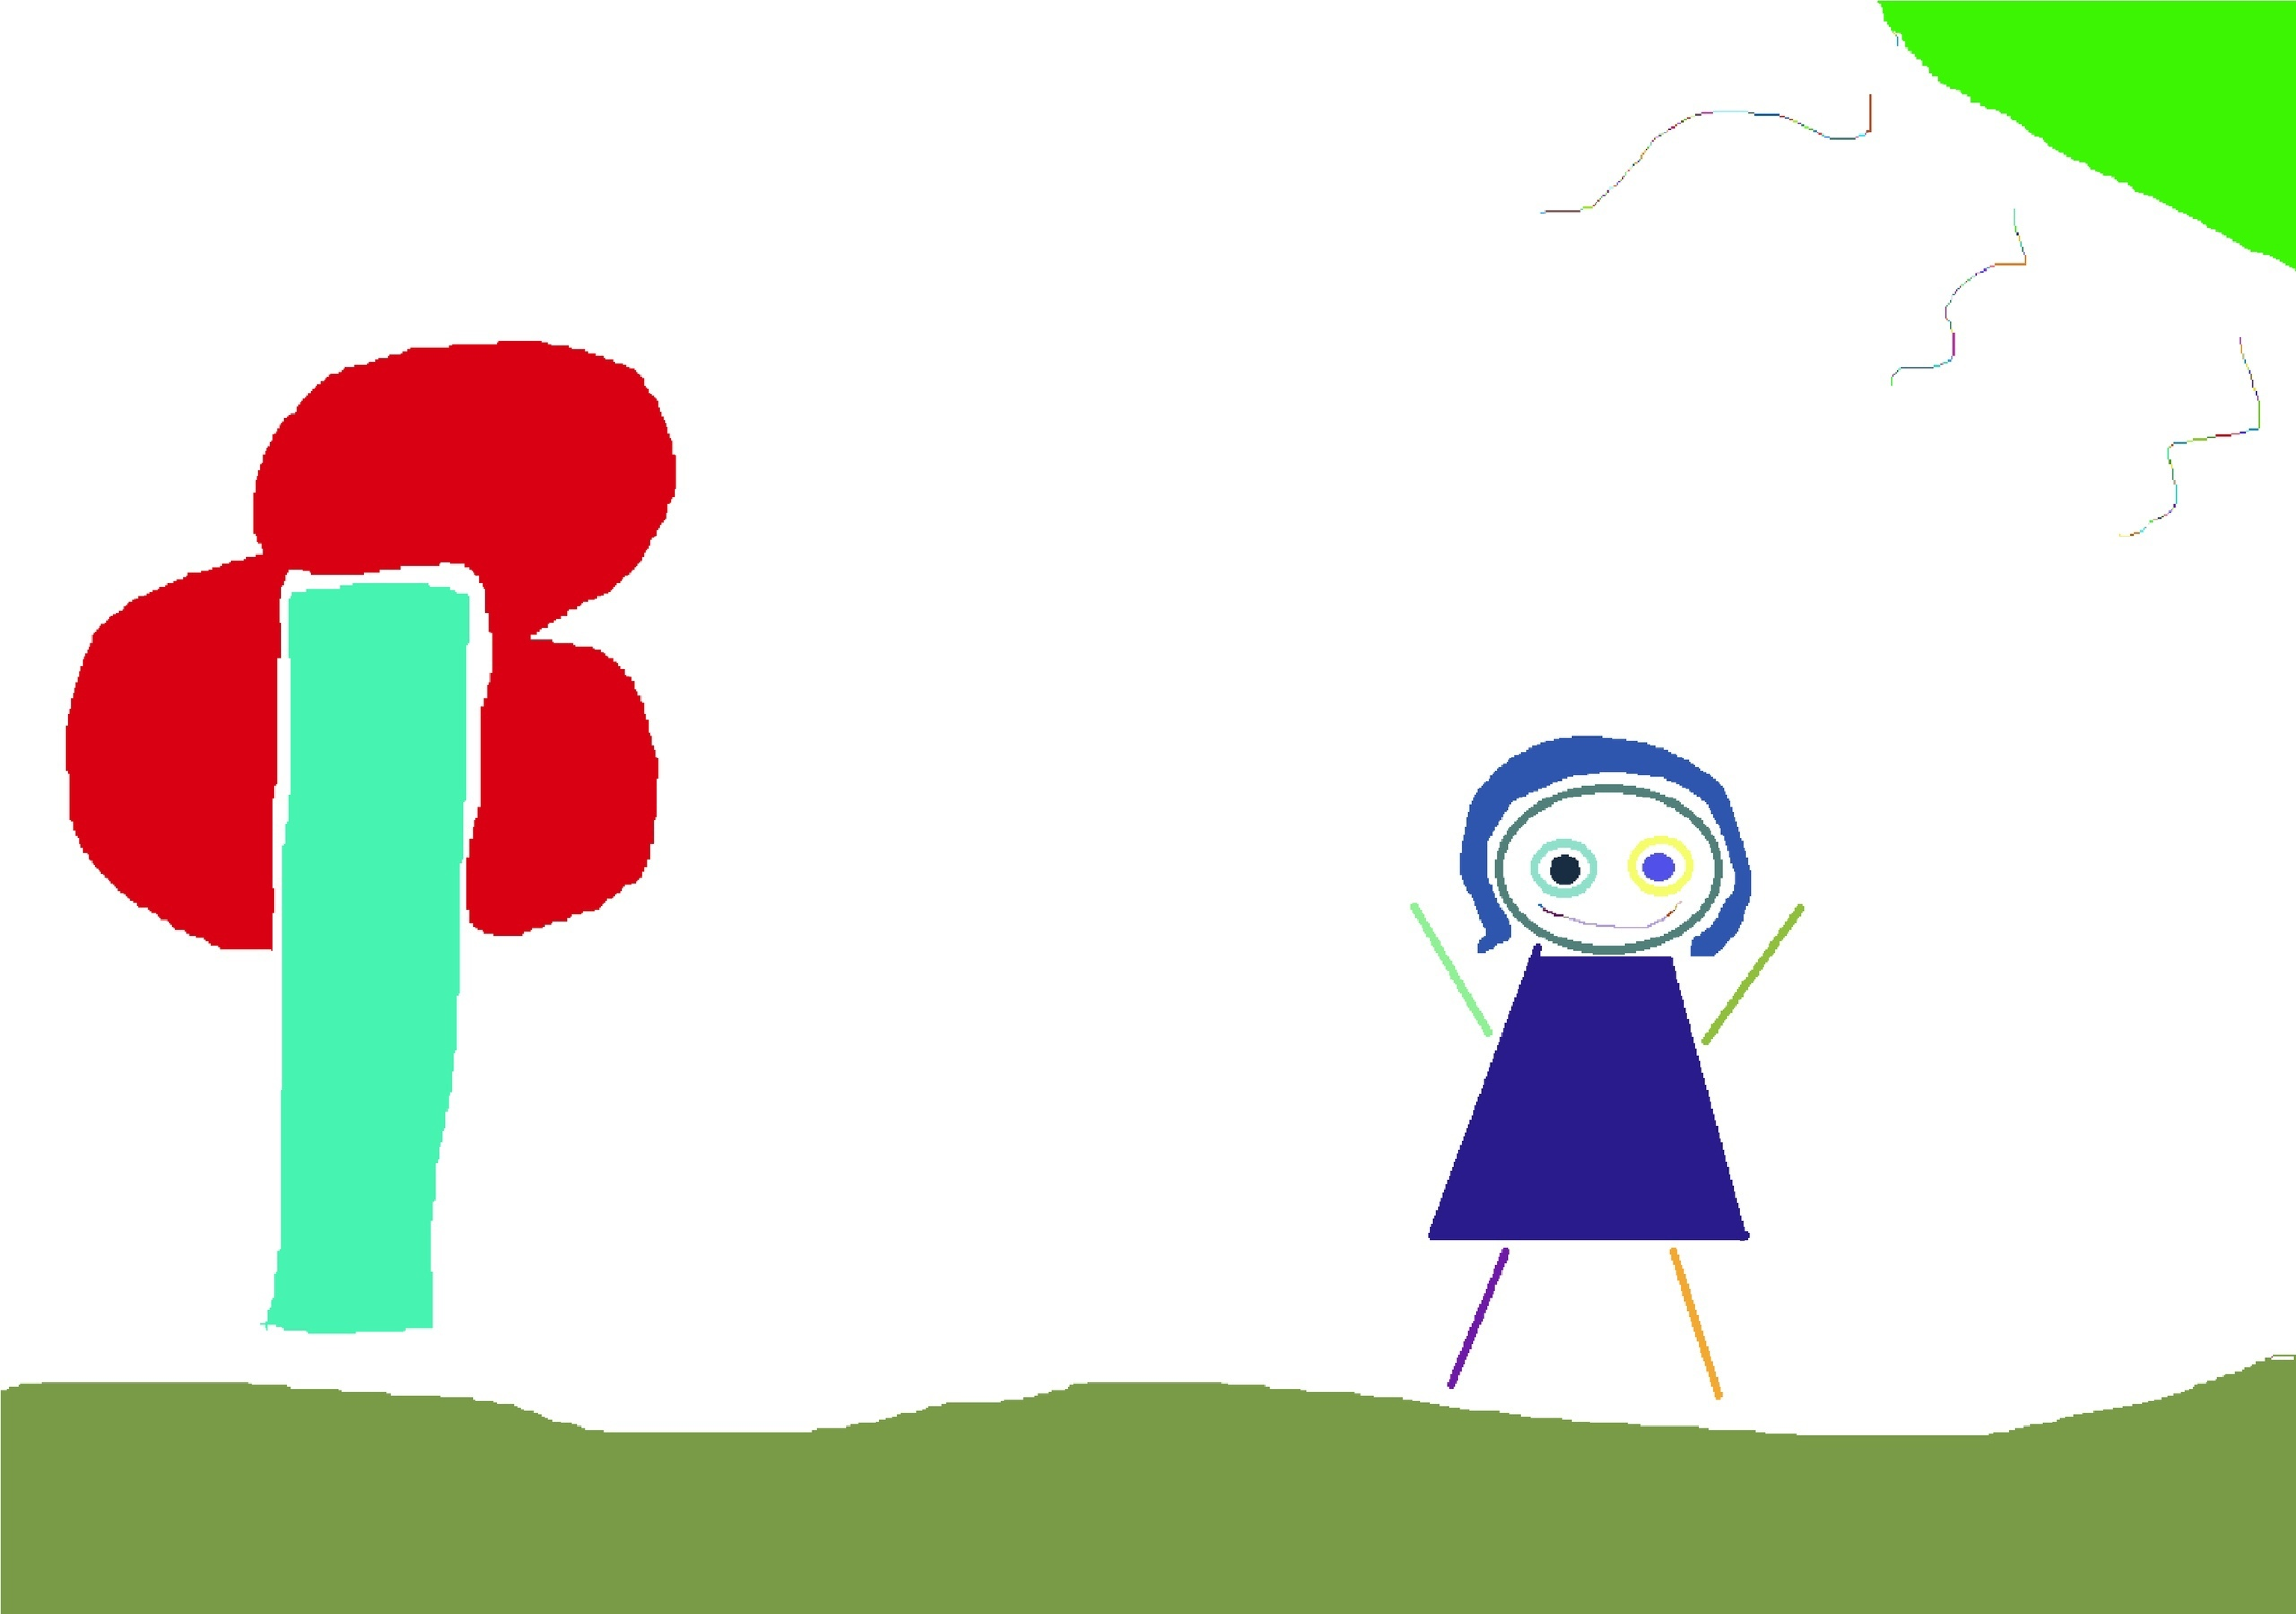
\includegraphics[scale=0.16]{girl_sec_dsu.pdf}}
\caption{Последовательный СНМ алгоритм}
\end{figure}
\begin{figure}[H]
\center{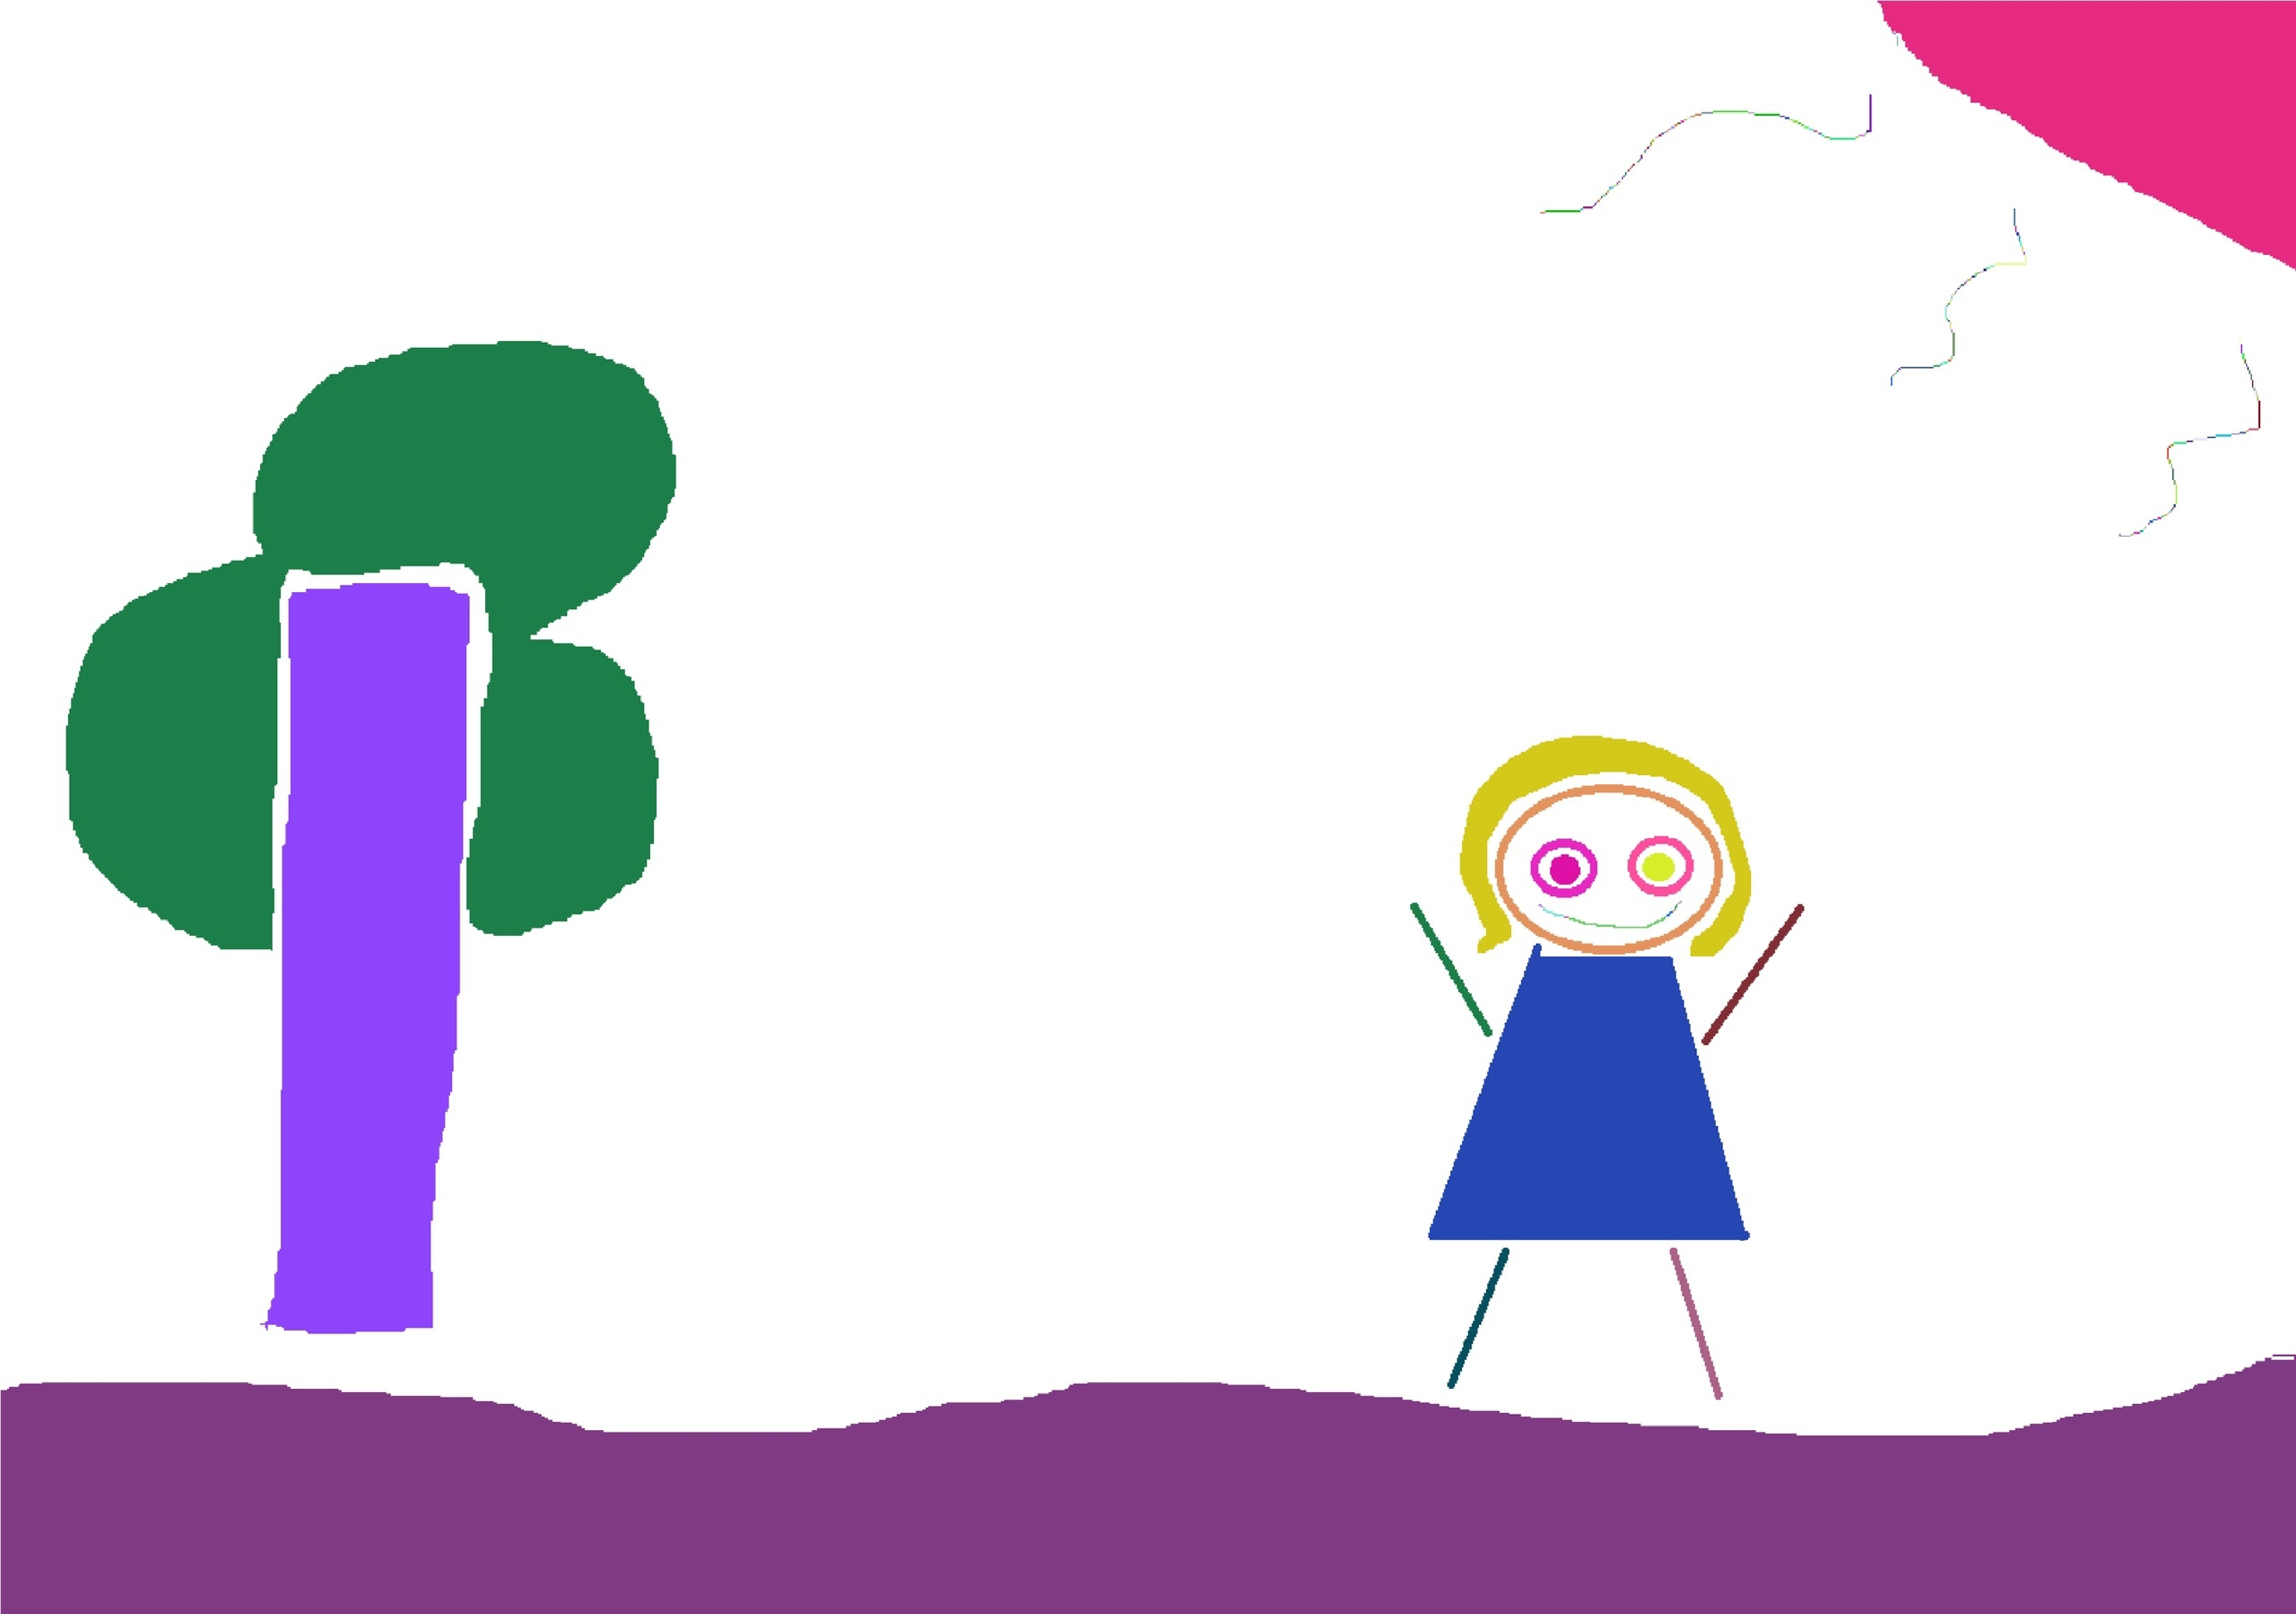
\includegraphics[scale=0.16]{girl_omp.pdf}}
\caption{Параллельный OMP алгоритм}
\end{figure}
\begin{figure}[H]
\center{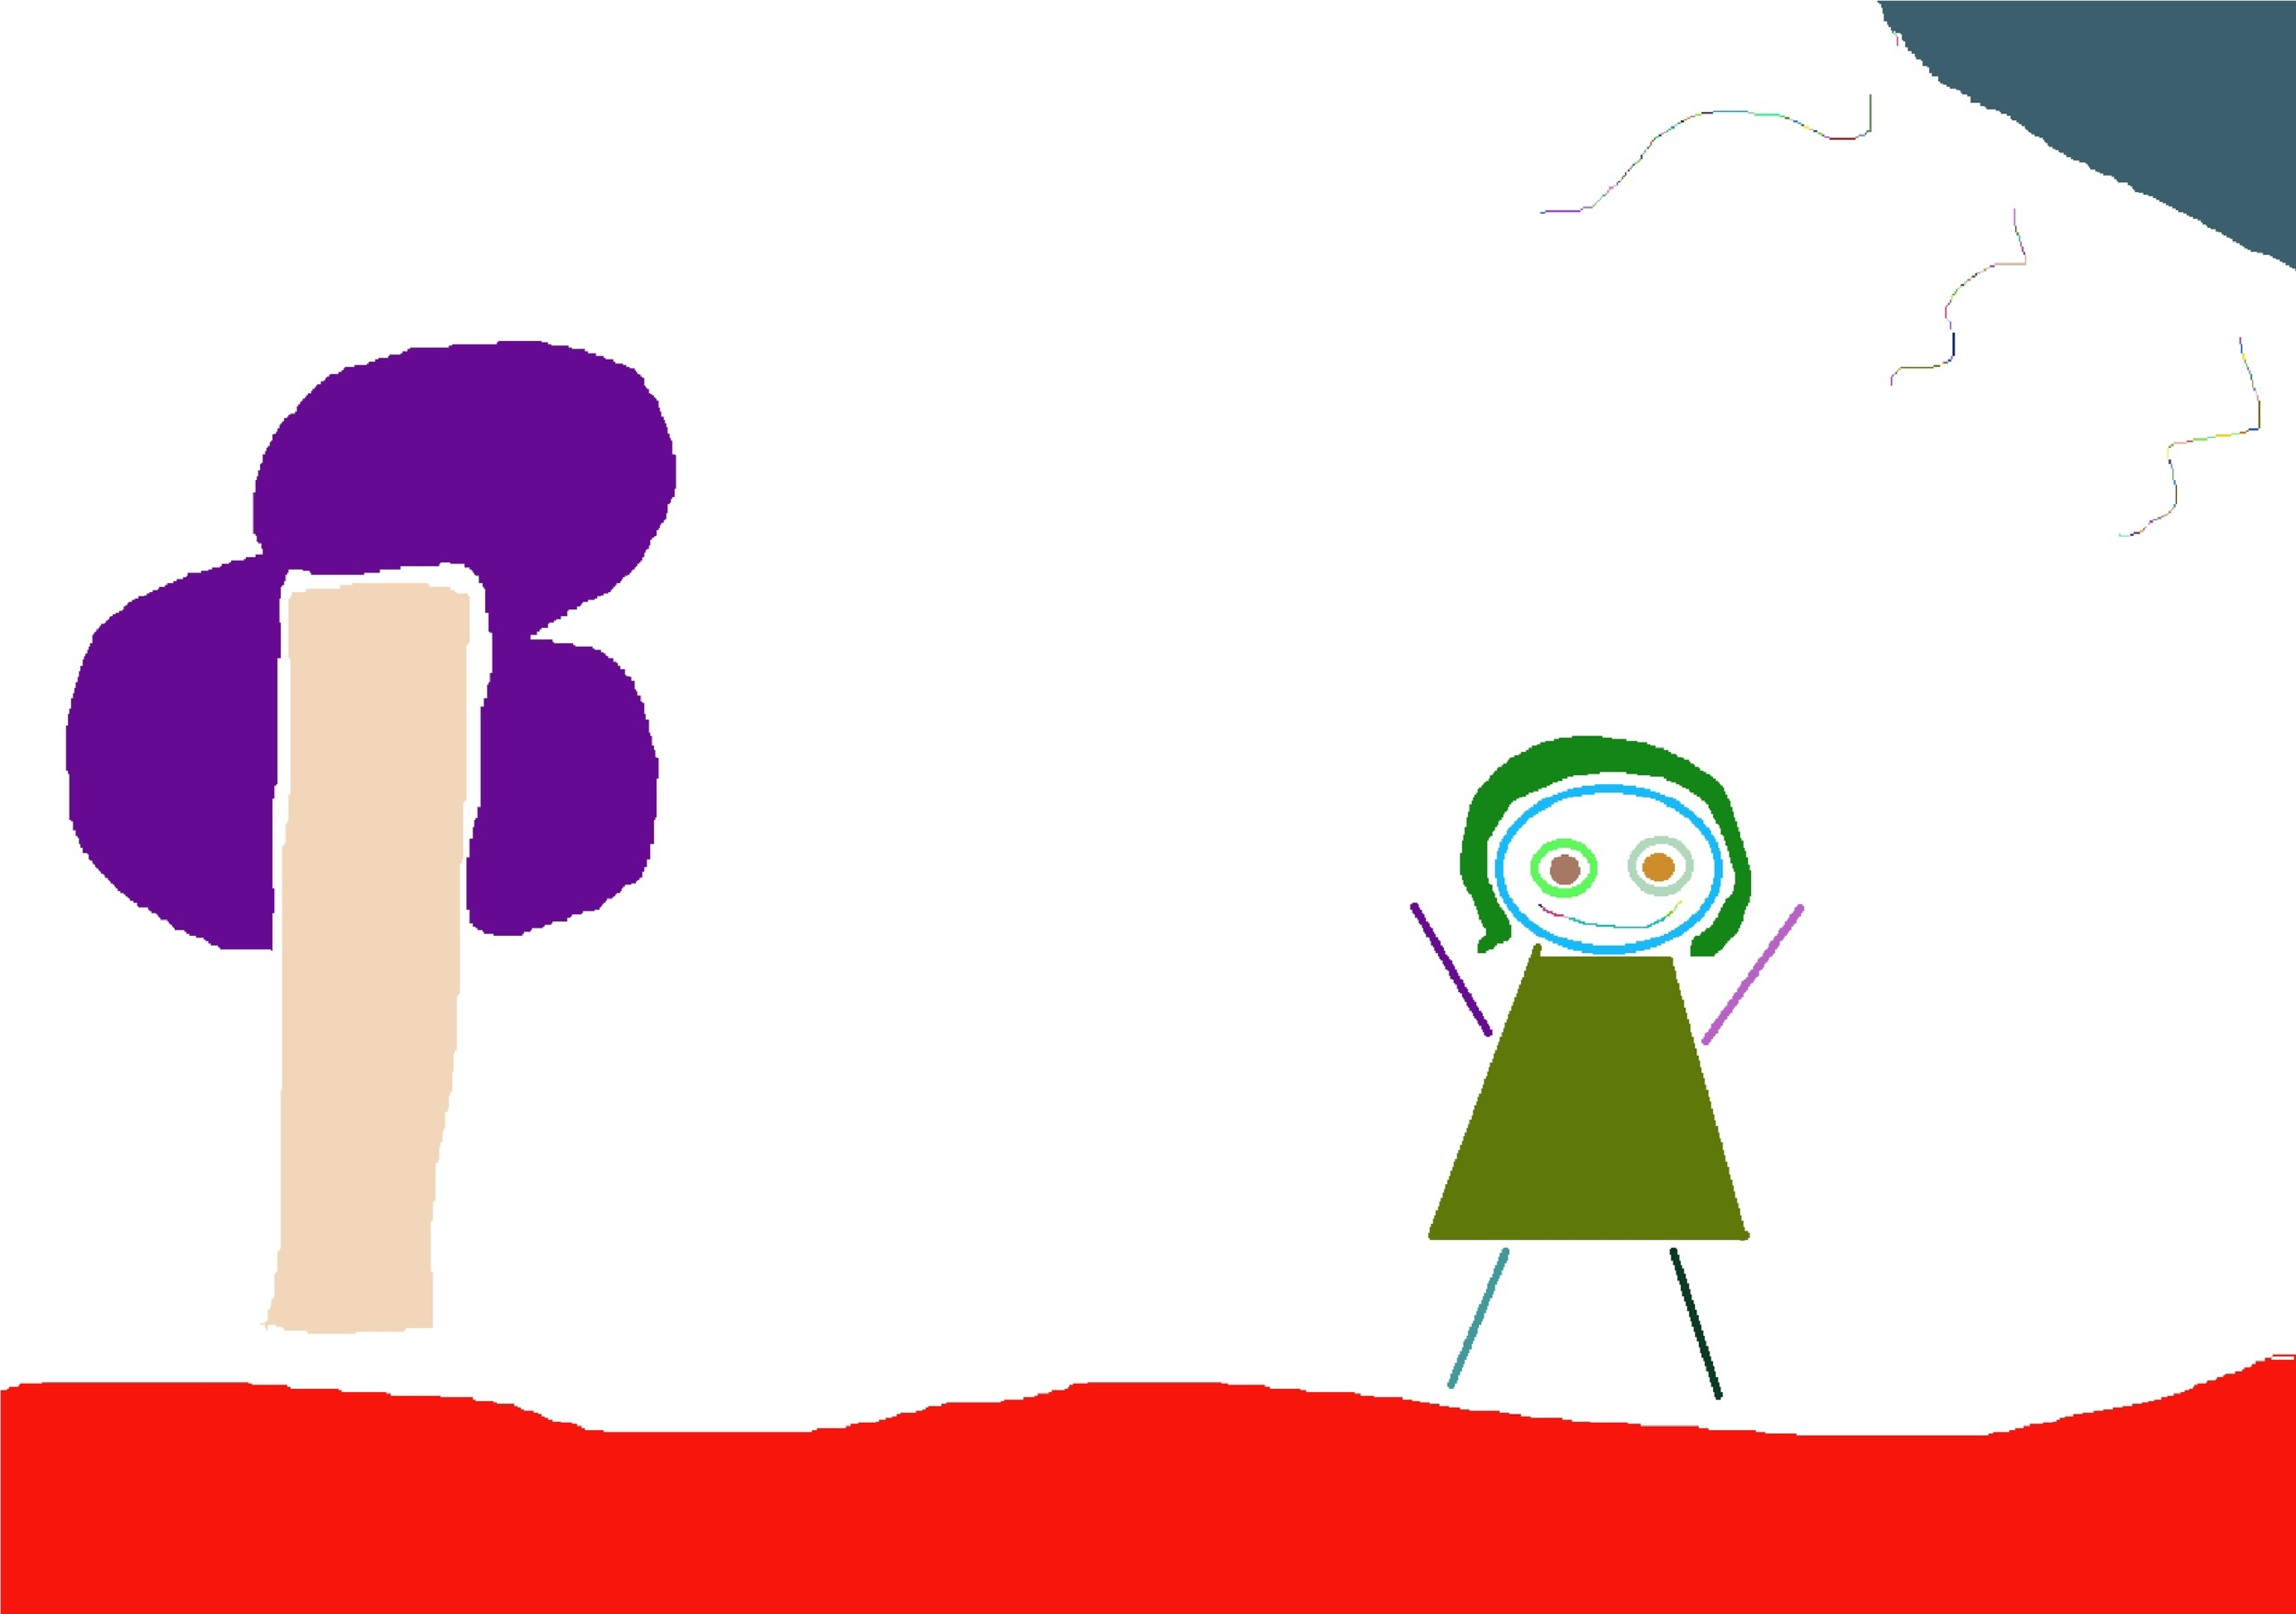
\includegraphics[scale=0.16]{girl_tbb.pdf}}
\caption{Параллельный TBB алгоритм}
\end{figure}
\begin{figure}[H]
\center{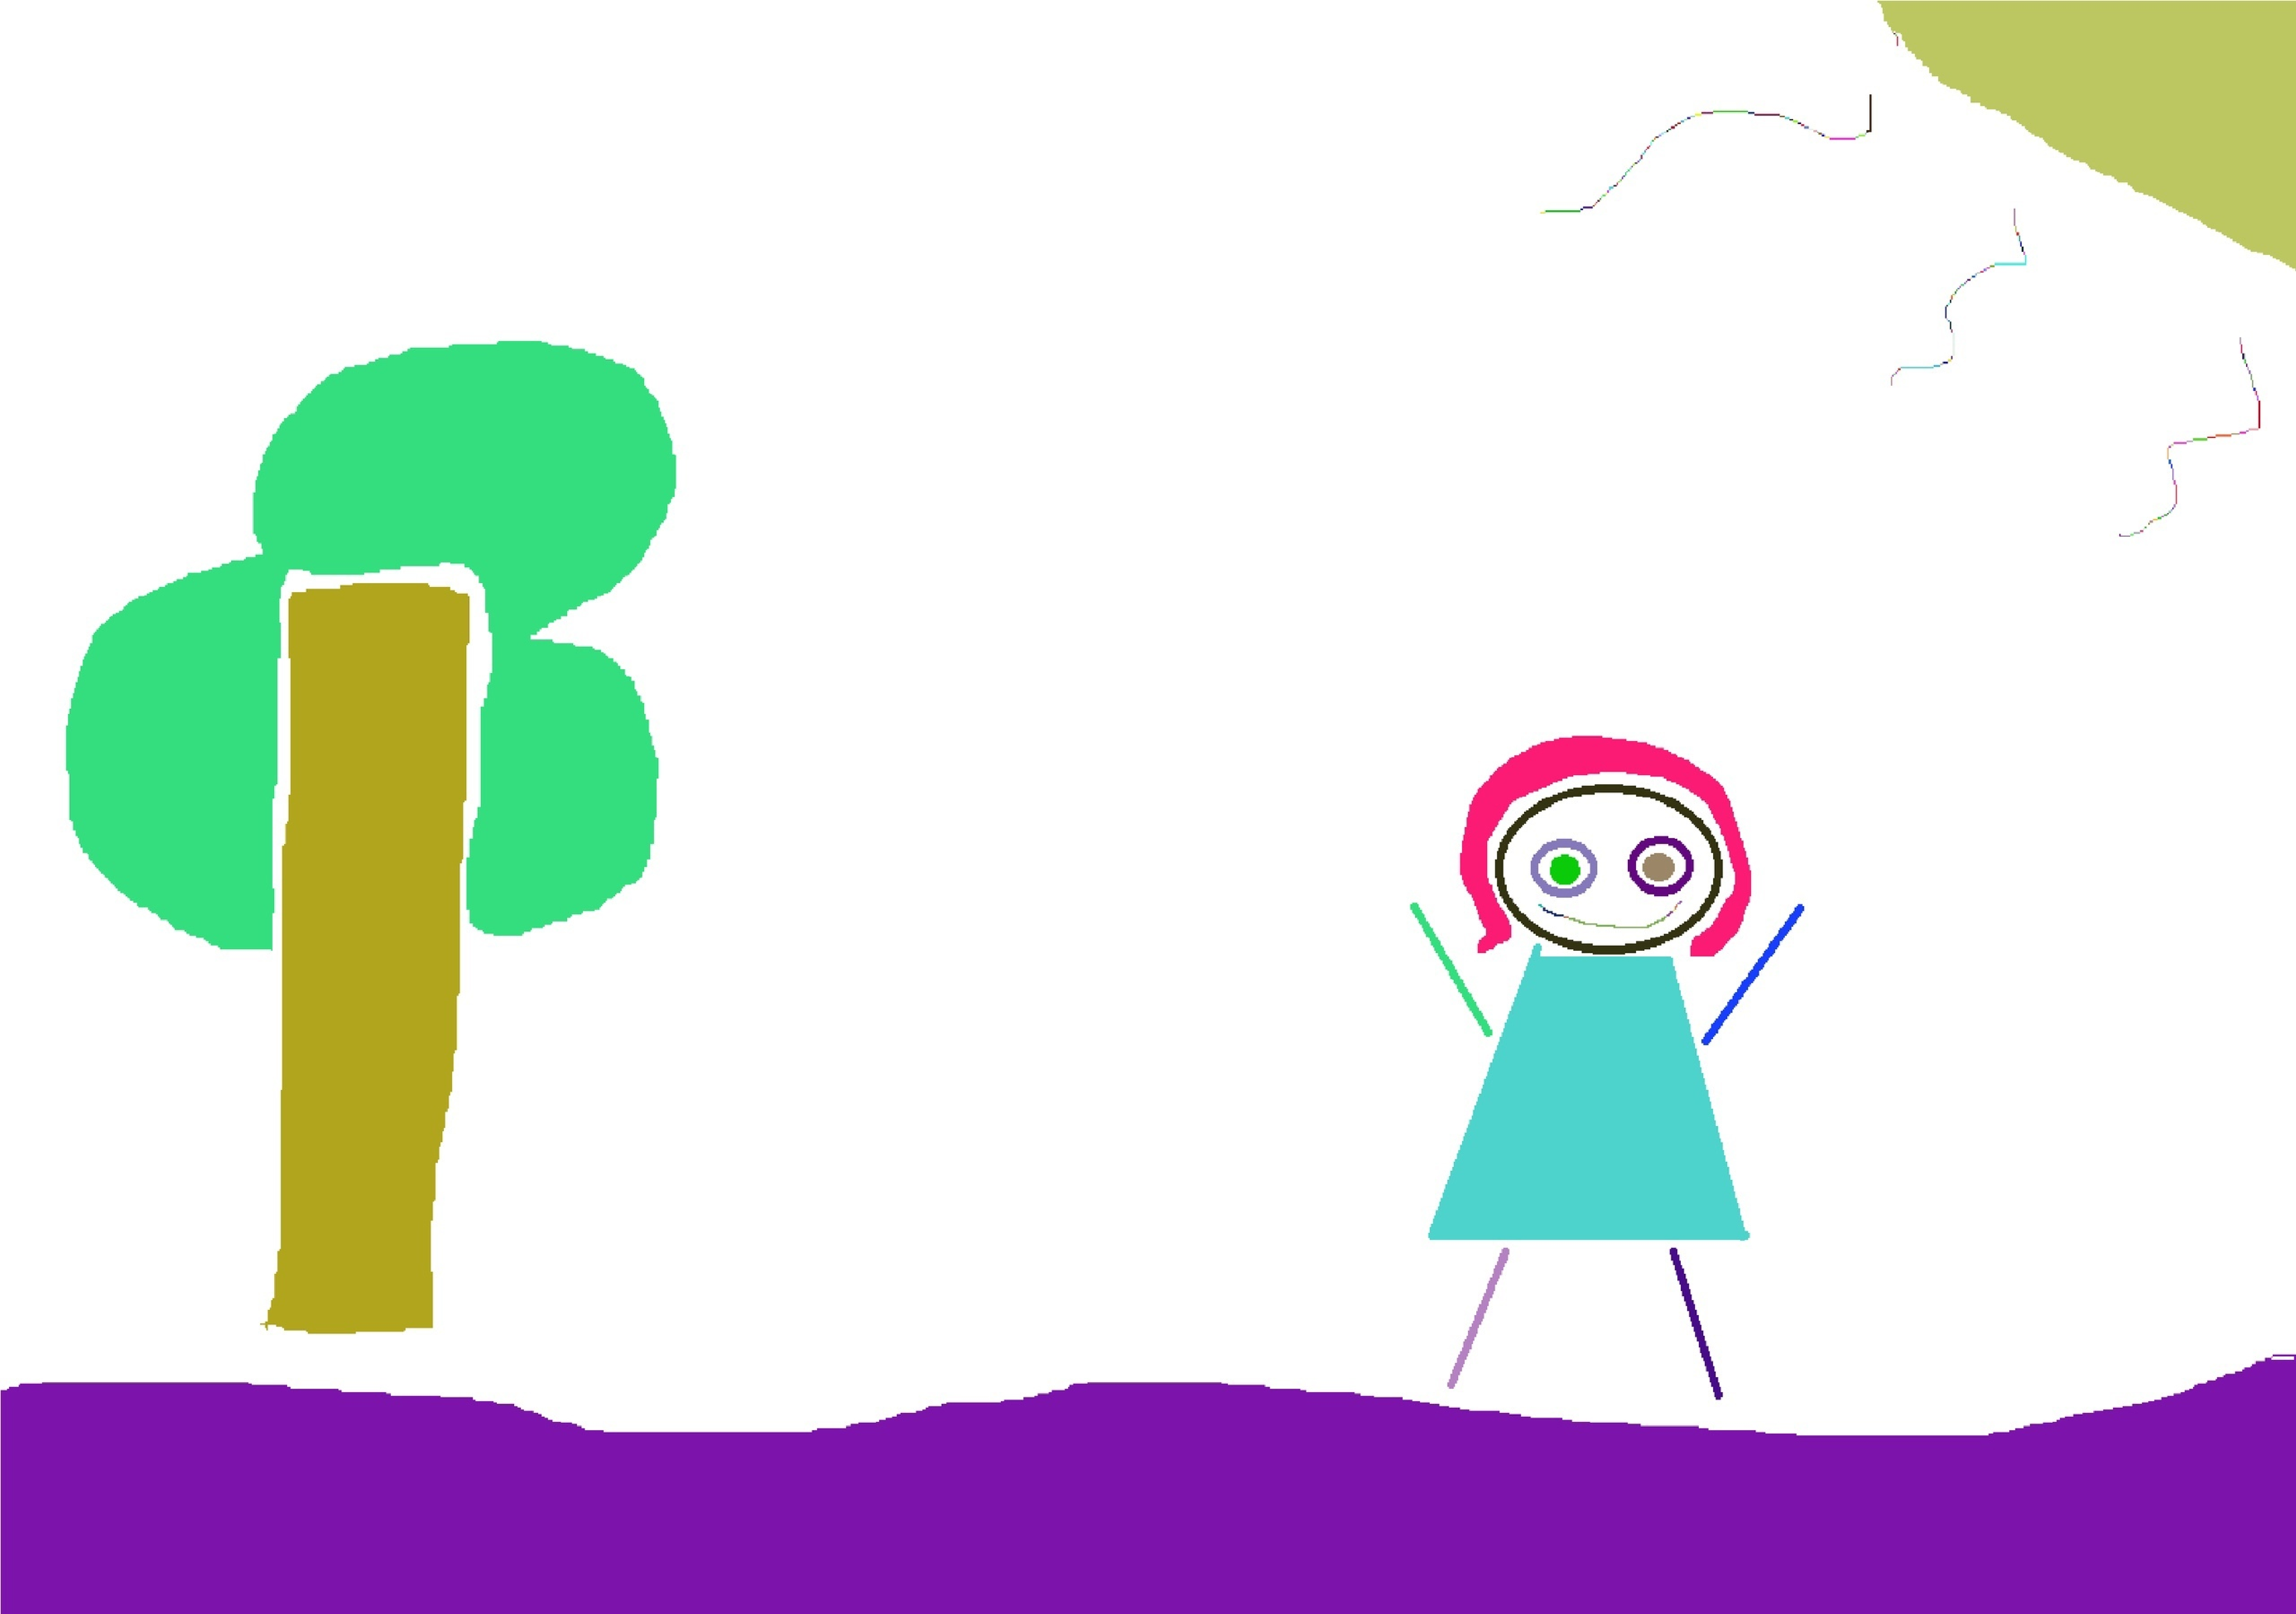
\includegraphics[scale=0.16]{girl_std.pdf}}
\caption{Параллельный STD:thread алгоритм}
\end{figure}

\subsection*{Пример на картинке с одной компонентой связности:} 

\begin{figure}[H]
\center{
\includegraphics[scale=0.7]{one_component_original.pdf}}
\caption{Оригинальное изображение}
\end{figure}
\begin{figure}[H]
\center{
\includegraphics[scale=0.75]{one_component_sec_bfs.pdf}}
\caption{Последовательный bfs алгоритм}
\end{figure}
\begin{figure}[H]
\center{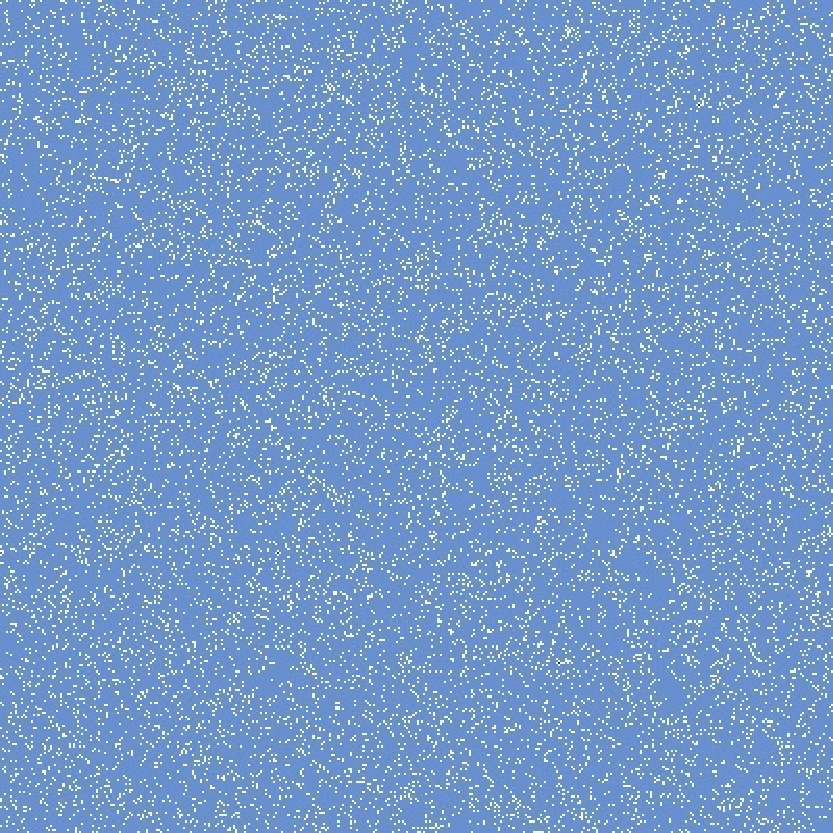
\includegraphics[scale=0.75]{one_component_sec_dsu.pdf}}
\caption{Последовательный СНМ алгоритм}
\end{figure}
\begin{figure}[H]
\center{
\includegraphics[scale=0.75]{one_component_omp.pdf}}
\caption{Параллельный OMP алгоритм}
\end{figure}
\begin{figure}[H]
\center{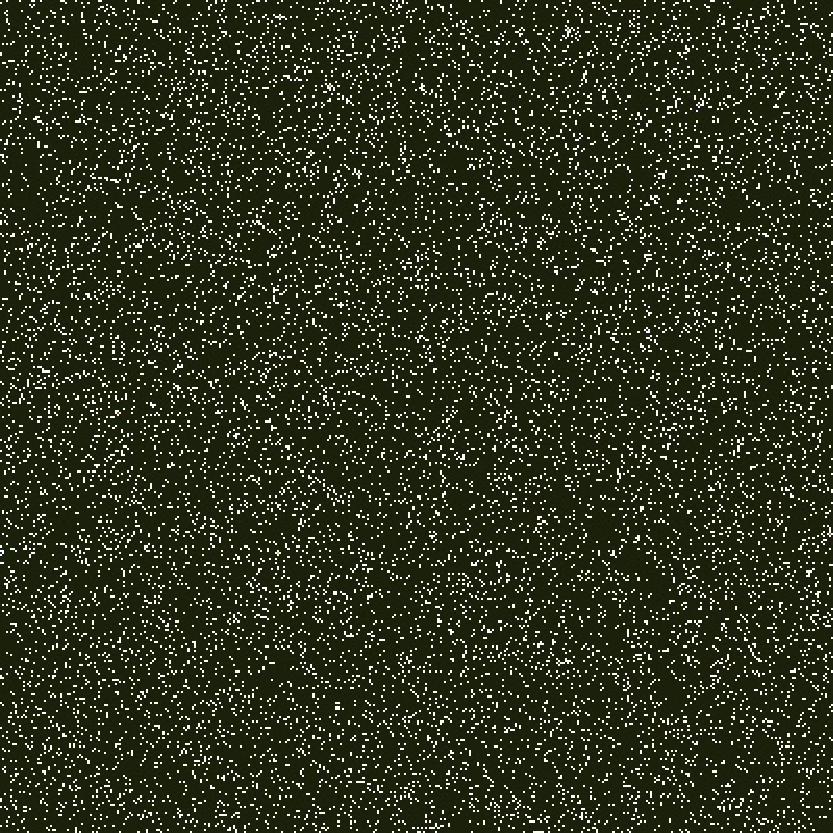
\includegraphics[scale=0.75]{one_component_tbb.pdf}}
\caption{Параллельный TBB алгоритм}
\end{figure}
\begin{figure}[H]
\center{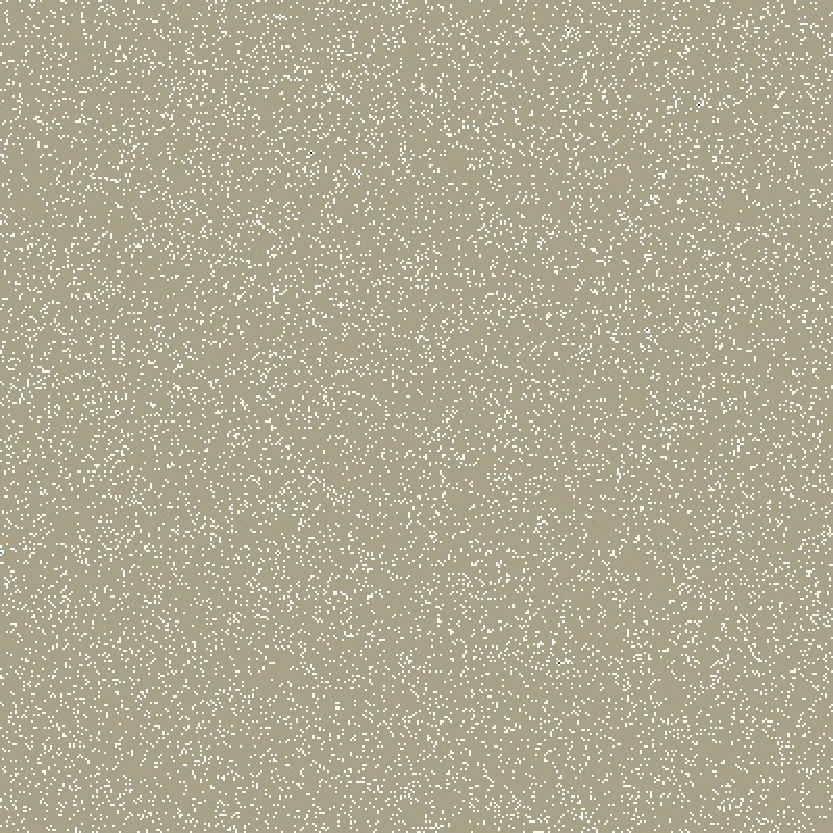
\includegraphics[scale=0.68]{one_component_std.pdf}}
\caption{Параллельный STD:thread алгоритм}
\end{figure}

\subsection*{Пример на картинке с большим количеством компонент связности:} 

\begin{figure}[H]
\center{
\includegraphics[scale=0.68]{a_lot_components_img_original.pdf}}
\caption{Оригинальное изображение}
\end{figure}
\begin{figure}[H]
\center{
\includegraphics[scale=0.75]{a_lot_components_img_sec_bfs.pdf}}
\caption{Последовательный bfs алгоритм}
\end{figure}
\begin{figure}[H]
\center{
\includegraphics[scale=0.75]{a_lot_components_img_sec_dsu.pdf}}
\caption{Последовательный СНМ алгоритм}
\end{figure}
\begin{figure}[H]
\center{
\includegraphics[scale=0.75]{a_lot_components_img_omp.pdf}}
\caption{Параллельный OMP алгоритм}
\end{figure}
\begin{figure}[H]
\center{
\includegraphics[scale=0.75]{a_lot_components_img_tbb.pdf}}
\caption{Параллельный TBB алгоритм}
\end{figure}
\begin{figure}[H]
\center{
\includegraphics[scale=0.75]{a_lot_components_img_std.pdf}}
\caption{Параллельный STD:thread алгоритм}
\end{figure}

\par Как видим, все наши алгоритмы работают корректно.

\newpage
\section*{Заключение}
\addcontentsline{toc}{section}{Заключение}
	\par В результате лабораторной работы были разработаны последовательные и параллельные реализации алгоритма маркировки компонент на бинарном изображении. Была проанализирована и продемонстрирована эффективность работы различных версий версий. Были разработаны тесты с использованием Google C++ Testing Framework, демонстрирующие корректность работы алгоритмов. Также была продемонстрирована корректность работы алгоритмов визуально с помощью библиотеки opencv.
\par Таким образом, все цели, поставленные в данной лабораторной работе, были успешно достигнуты.

\newpage
% \section*{Литература}
% \addcontentsline{toc}{section}{Литература}
\begin{thebibliography}{1}
\addcontentsline{toc}{section}{Литература}
\bibitem{Sterjanov} Стержанов М., «Методики выделения связных компонент в штриховых бинарных изображениях». Минск
\bibitem{Kornyakov} Корняков К.В., Кустикова В.Д., Мееров И.Б., Сиднев А.А., Сысоев А.В., Шишков А.В., «Инструменты параллельного программирования в системах с общей памятью», Нижний Новгород, 2010.
\bibitem{Gergel} Гергель В.П., «Введение в методы параллельного
программирования. Параллельное программирование с использованием
OpenMP», Нижний Новгород, 2007.
\bibitem{E-maxx} E-maxx: Система непересекающихся множеств [Электронный ресурс] // URL: \url{https://e-maxx.ru/algo/dsu}
\bibitem{habr} Habr: Потоки, блокировки и условные переменные в C++11 [Электронный ресурс] // URL: \url{https://habr.com/ru/post/182610/}
\end{thebibliography}
\newpage
\section*{Приложение}
\addcontentsline{toc}{section}{Приложение}
\par В этом разделе находится листинг кода.
\par Последовательные реализации и класс системы непересекающихся множеств ($Disjoint\_Set\_Union$):
\begin{lstlisting}

Disjoint_Set_Union.h

// Copyright 2021 Oganyan Robert

#ifndef MODULES_TASK_2_OGANYAN_R_MARK_COMPONENTS_OMP_DISJOINT_SET_UNION_H_
#define MODULES_TASK_2_OGANYAN_R_MARK_COMPONENTS_OMP_DISJOINT_SET_UNION_H_


#include <vector>
#include <iostream>
#include <utility>
#include <algorithm>
#include <tbb/parallel_for.h>
#include <tbb/blocked_range2d.h>
#include <tbb/task_scheduler_init.h>
#include "../../3rdparty/unapproved/unapproved.h"
#include <omp.h>

template<typename T>
class Disjoint_Set_Union {
private:
    std::vector<T> rank;
    std::vector<T> parent;

public:
    explicit Disjoint_Set_Union(int size) : rank(size), parent(size) {
    }

    void make_set(int vertex) {
        parent[vertex] = vertex;
        rank[vertex] = 0;
    }


    void Init() {
        for (std::size_t vertex = 0; vertex < rank.size(); ++vertex) {
            make_set(vertex);
        }
    }

    void InitOmp(int num_proc) {
        omp_set_num_threads(num_proc);
#pragma omp parallel default(none) shared(parent, rank)
        {
#pragma omp for schedule(static)
            for (std::size_t vertex = 0; vertex < rank.size(); ++vertex) {
                make_set(vertex);
            }
        }
        return;
    }

    void InitTbb(int num_proc) {
        tbb::task_scheduler_init init(num_proc);
        tbb::parallel_for(tbb::blocked_range<int>(0, rank.size(),
        rank.size() / num_proc + 1),
                          [&](tbb::blocked_range<int> block) {
                              for (auto vertex = block.begin();
                              vertex != block.end(); ++vertex) {
                                  make_set(vertex);
                              }
                          });

        init.terminate();
    }

    void InitStd(int num_proc) {
        std::vector<std::thread> threads;
        threads.reserve(num_proc);
        int div = rank.size() / num_proc;
        int mod = rank.size() % num_proc;

        int last = 0;


        for (int proc = 0; proc < num_proc; ++proc) {
            threads.emplace_back([&, proc, div, mod, last]() {
                int balance = (proc < mod) ? 1 : 0;
                for (int vertex = last; vertex < last + div + balance; ++vertex) {
                    make_set(vertex);
                }
            });
            last += div + ((proc < mod) ? 1 : 0);
        }

        for (auto &thread : threads) {
            thread.join();
        }

    }

    /*
    void Init(int size) {
        rank.resize(size);
        parent.resize(size);
        for (int vertex = 0; vertex < size; ++vertex) {
            make_set(vertex);
        }
    }
    */

    int find_set(int vertex) {
        //  Bug here (parent[vertex] = [parent[paren[vertex]])
        if (vertex == parent[vertex]) {
            return vertex;
        }

        return parent[vertex] = find_set(parent[vertex]);
    }

    int find_set(int vertex, int last) {
        if (vertex == parent[vertex]) {
            return vertex;
        }

        if (last == parent[vertex]) {
            return std::min(last, vertex);
        }

        return parent[vertex] = find_set(parent[vertex], vertex);
    }

    void union_sets(int fi_union, int se_union) {
        fi_union = find_set(fi_union, fi_union);
        se_union = find_set(se_union, se_union);
        if (fi_union != se_union) {
            if (rank[fi_union] < rank[se_union])
                std::swap(fi_union, se_union);
            parent[se_union] = fi_union;
            if (rank[fi_union] == rank[se_union])
                ++rank[fi_union];
        }
    }

    const std::vector<T> get_rank() {
        return this->rank;
    }

    const std::vector<T> get_parent() {
        return this->parent;
    }
};

#endif  //  MODULES_TASK_2_OGANYAN_R_MARK_COMPONENTS_OMP_DISJOINT_SET_UNION_H_

mark_components_seq.h

#ifndef MODULES_TASK_1_OGANYAN_R_MARK_COMPONENTS_MARK_COMPONENTS_SEQ_H_
#define MODULES_TASK_1_OGANYAN_R_MARK_COMPONENTS_MARK_COMPONENTS_SEQ_H_

#include <vector>
#include <cstdint>
#include <queue>
#include <stdexcept>
#include <utility>
#include "Disjoint_Set_Union.h"


int MarkComponentsSeq(std::vector<int> *img,
                      int height, int width);

#endif  //  MODULES_TASK_1_OGANYAN_R_MARK_COMPONENTS_MARK_COMPONENTS_SEQ_H_


mark_components_seq.cpp

#include "../../modules/task_1/oganyan_r_mark_components/mark_components_seq.h"

static const std::vector<std::pair<int, int>> directions{
        // {-1, -1},
        {-1, 0},
        //  {-1, 1},
        {0,  -1},
        {0,  1},
        // {1,  -1},
        {1,  0},
        // {1,  1},
};


int MarkComponentsSeq(std::vector<int> *img_new, int height, int width) {
    if ((*img_new).size() == 0) {
        throw std::invalid_argument("Size of the image cant be negative");
    }
    if (static_cast<int>((*img_new).size()) != width * height) {
        throw std::invalid_argument("Size of the image is not correct");
    }
    int count_comp{0};
    Disjoint_Set_Union<int> dsu(height * width);
    dsu.Init();

    for (int i = 0; i < height; ++i) {
        for (int j = 0; j < width; ++j) {
            if ((*img_new)[i * width + j]) {
                for (auto &neighbor : directions) {
                    if (i + neighbor.first >= height || i + neighbor.first < 0
                        || j + neighbor.second >= width ||
                        j + neighbor.second < 0) {
                        continue;
                    }
                    int cur = (i + neighbor.first) * width + j + neighbor.second;
                    if ((*img_new)[cur] == 0) {
                        continue;
                    }
                    dsu.union_sets(i * width + j, cur);
                }
            }
        }
    }

    for (int i = 0; i < height; ++i) {
        for (int j = 0; j < width; ++j) {
            int cur = i * width + j;
            if ((*img_new)[cur]) {
                (*img_new)[cur] = dsu.find_set(cur, cur) + 1;
            }
            if ((*img_new)[cur] == cur + 1) {
                count_comp++;
            }
        }
    }

    return count_comp;
}

mark_components_seq_bfs.h

// Copyright 2021 Oganyan Robert


#ifndef MODULES_TASK_1_OGANYAN_R_MARK_COMPONENTS_MARK_COMPONENTS_H_
#define MODULES_TASK_1_OGANYAN_R_MARK_COMPONENTS_MARK_COMPONENTS_H_

#include <vector>
#include <cstdint>
#include <queue>
#include <stdexcept>
#include <utility>

int MarkComponentsSeqBfs(std::vector<int> *img,
                   int height, int width);


void bfs(std::vector<int> *img, std::pair<int, int> start,
         int *number, int width, int height);

#endif  //  MODULES_TASK_1_OGANYAN_R_MARK_COMPONENTS_MARK_COMPONENTS_H_


mark_components_seq_bfs.cpp

// Copyright 2021 Oganyan Robert

#include <iostream>
#include "../../modules/task_1/oganyan_r_mark_components/mark_components_seq_bfs.h"

static const std::vector<std::pair<int, int>> directions{
        {-1, 0},
        {0,  -1},
        {0,  1},
        {1,  0},
};


void bfs(std::vector<int> *img, std::pair<int, int> start,
           int *number, int width, int height) {
    if ((*img)[start.first * width + start.second] != 1) {
        return;
    }
    std::queue<std::pair<int, int>> q;
    q.push({start});
    (*img)[start.first * width + start.second] = ++(*number);
    while (!q.empty()) {
        auto cur{q.front()};
        q.pop();
        for (auto &neighbor : directions) {
            if (cur.first + neighbor.first >= height || 
            cur.first + neighbor.first < 0
                || cur.second + neighbor.second >= width || 
                cur.second + neighbor.second < 0) {
                continue;
            }
            if ((*img)[(cur.first + neighbor.first) * width
            + cur.second + neighbor.second] == 1) {
                q.push({(cur.first + neighbor.first), cur.second
                + neighbor.second});
                (*img)[(cur.first + neighbor.first) * width
                + cur.second + neighbor.second] = (*number);
            }
        }
    }
    return;
}


int MarkComponentsSeqBfs(std::vector<int> *img, int height, int width) {
    if ((*img).size() == 0) {
        throw std::invalid_argument("Size of the image cant be negative");
    }
    if (static_cast<int>((*img).size()) != width * height) {
        throw std::invalid_argument("Size of the image is not correct");
    }
    int count_comp{1};
    for (int i{0}; i < height; ++i) {
        for (int j{0}; j < width; ++j) {
            bfs(img, {i, j}, &count_comp, width, height);
        }
    }
    return count_comp - 1;
}

main.cpp

// Copyright 2021 Oganyan Robert

#include <gtest/gtest.h>
#include <vector>
#include <random>
#include <chrono>
#include "../../modules/task_1/oganyan_r_mark_components/mark_components_seq_bfs.h"
#include "mark_components_seq.h"


TEST(Comparing_to_a_sample, rectangle_image) {
    uint16_t width = 3;
    uint16_t height = 5;
    std::vector<int> source_image{
            0, 1, 1,
            0, 0, 0,
            1, 1, 1,
            0, 1, 0,
            0, 0, 0,
    };
    std::vector<int> result_image{
            0, 2, 2,
            0, 0, 0,
            3, 3, 3,
            0, 3, 0,
            0, 0, 0,
    };
    int res_image;
    ASSERT_NO_THROW(res_image = MarkComponentsSeqBfs(&source_image,
    height, width));
    ASSERT_EQ(res_image, 2);
}

TEST(Wrong_data, wrong_img_2) {
    std::vector<int> source_image{};
    std::vector<int> result_image{};
    uint16_t width = 5;
    uint16_t height = 2;
    ASSERT_ANY_THROW(MarkComponentsSeqBfs(&source_image, height, width));
}


TEST(Comparing_to_a_sample, square_image_1) {
    uint16_t width = 6;
    uint16_t height = 6;
    std::vector<int> source_image{
            0, 1, 0, 0, 0, 0,
            1, 1, 1, 0, 0, 1,
            0, 0, 0, 0, 1, 1,
            0, 1, 0, 1, 0, 0,
            1, 1, 1, 0, 0, 0,
            0, 0, 0, 0, 1, 1,
    };
    std::vector<int> result_image{
            0, 2, 0, 0, 0, 0,
            2, 2, 2, 0, 0, 3,
            0, 0, 0, 0, 3, 3,
            0, 4, 0, 5, 0, 0,
            4, 4, 4, 0, 0, 0,
            0, 0, 0, 0, 6, 6,
    };
    int res_image;
    ASSERT_NO_THROW(res_image = MarkComponentsSeqBfs(&source_image,
    height, width));
    ASSERT_EQ(res_image, 5);
}

TEST(Wrong_data, wrong_width_and_height_3) {
    std::vector<int> source_image{
            0, 0, 1,
            1, 0, 1,
            0, 0, 0,
    };
    std::vector<int> result_image{
            0, 0, 2,
            3, 0, 2,
            0, 0, 0,
    };
    uint16_t width = 1;
    uint16_t height = 3;
    ASSERT_ANY_THROW(MarkComponentsSeqBfs(&source_image, height, width));
}

TEST(Comparing_to_a_big_sample, square_image_1) {
    uint16_t width = 15;
    uint16_t height = 15;
    std::vector<int> source_image{
            1, 1, 1, 1, 1, 1, 1, 1, 1, 1, 1, 1, 1, 1, 1,
            1, 1, 1, 1, 1, 1, 1, 1, 1, 1, 1, 1, 1, 1, 1,
            1, 1, 1, 1, 1, 1, 1, 1, 1, 1, 1, 1, 1, 1, 1,
            1, 1, 1, 1, 1, 1, 1, 1, 1, 1, 1, 1, 1, 1, 1,
            1, 1, 1, 1, 1, 1, 1, 1, 1, 1, 1, 1, 1, 1, 1,
            1, 1, 1, 1, 1, 1, 1, 1, 1, 1, 1, 1, 1, 1, 1,
            1, 1, 1, 1, 1, 1, 1, 1, 1, 1, 1, 1, 1, 1, 1,
            1, 1, 1, 1, 1, 1, 1, 1, 1, 1, 1, 1, 1, 1, 1,
            1, 1, 1, 1, 1, 1, 1, 1, 1, 1, 1, 1, 1, 1, 1,
            1, 1, 1, 1, 1, 1, 1, 1, 1, 1, 1, 1, 1, 1, 1,
            1, 1, 1, 1, 1, 1, 1, 1, 1, 1, 1, 1, 1, 1, 1,
            1, 1, 1, 1, 1, 1, 1, 1, 1, 1, 1, 1, 1, 1, 1,
            1, 1, 1, 1, 1, 1, 1, 1, 1, 1, 1, 1, 1, 1, 1,
            1, 1, 1, 1, 1, 1, 1, 1, 1, 1, 1, 1, 1, 1, 1,
            1, 1, 1, 1, 1, 1, 1, 1, 1, 1, 1, 1, 1, 1, 1,
    };
    std::vector<int> result_image{
            2, 2, 2, 2, 2, 2, 2, 2, 2, 2, 2, 2, 2, 2, 2,
            2, 2, 2, 2, 2, 2, 2, 2, 2, 2, 2, 2, 2, 2, 2,
            2, 2, 2, 2, 2, 2, 2, 2, 2, 2, 2, 2, 2, 2, 2,
            2, 2, 2, 2, 2, 2, 2, 2, 2, 2, 2, 2, 2, 2, 2,
            2, 2, 2, 2, 2, 2, 2, 2, 2, 2, 2, 2, 2, 2, 2,
            2, 2, 2, 2, 2, 2, 2, 2, 2, 2, 2, 2, 2, 2, 2,
            2, 2, 2, 2, 2, 2, 2, 2, 2, 2, 2, 2, 2, 2, 2,
            2, 2, 2, 2, 2, 2, 2, 2, 2, 2, 2, 2, 2, 2, 2,
            2, 2, 2, 2, 2, 2, 2, 2, 2, 2, 2, 2, 2, 2, 2,
            2, 2, 2, 2, 2, 2, 2, 2, 2, 2, 2, 2, 2, 2, 2,
            2, 2, 2, 2, 2, 2, 2, 2, 2, 2, 2, 2, 2, 2, 2,
            2, 2, 2, 2, 2, 2, 2, 2, 2, 2, 2, 2, 2, 2, 2,
            2, 2, 2, 2, 2, 2, 2, 2, 2, 2, 2, 2, 2, 2, 2,
            2, 2, 2, 2, 2, 2, 2, 2, 2, 2, 2, 2, 2, 2, 2,
            2, 2, 2, 2, 2, 2, 2, 2, 2, 2, 2, 2, 2, 2, 2,
    };
    int res_image;
    ASSERT_NO_THROW(res_image = MarkComponentsSeqBfs(&source_image,
    height, width));
    ASSERT_EQ(res_image, 1);
}

TEST(Wrong_data, wrong_width_and_height_1) {
    std::vector<int> source_image = {
            0, 1, 1,
            1, 0, 0,
            0, 0, 0,
    };
    std::vector<int> result_image = {
            0, 2, 2,
            3, 0, 0,
            0, 0, 0,
    };
    uint16_t width = 4;
    uint16_t height = 3;
    ASSERT_ANY_THROW(MarkComponentsSeqBfs(&source_image, height, width));
}

TEST(Comparing_to_a_big_sample, square_image_2) {
    uint16_t width = 10;
    uint16_t height = 10;
    std::vector<int> source_image{
            1, 1, 1, 1, 1, 1, 1, 1, 1, 1,
            1, 0, 0, 0, 0, 0, 0, 0, 0, 1,
            1, 0, 1, 1, 1, 1, 1, 1, 0, 1,
            1, 0, 1, 0, 0, 0, 0, 1, 0, 1,
            1, 0, 1, 0, 1, 1, 0, 1, 0, 1,
            1, 0, 1, 0, 1, 1, 0, 1, 0, 1,
            1, 0, 1, 0, 0, 0, 0, 1, 0, 1,
            1, 0, 1, 1, 1, 1, 1, 1, 0, 1,
            1, 0, 0, 0, 0, 0, 0, 0, 0, 1,
            1, 1, 1, 1, 1, 1, 1, 1, 1, 1,
    };
    std::vector<int> result_image{
            2, 2, 2, 2, 2, 2, 2, 2, 2, 2,
            2, 0, 0, 0, 0, 0, 0, 0, 0, 2,
            2, 0, 3, 3, 3, 3, 3, 3, 0, 2,
            2, 0, 3, 0, 0, 0, 0, 3, 0, 2,
            2, 0, 3, 0, 4, 4, 0, 3, 0, 2,
            2, 0, 3, 0, 4, 4, 0, 3, 0, 2,
            2, 0, 3, 0, 0, 0, 0, 3, 0, 2,
            2, 0, 3, 3, 3, 3, 3, 3, 0, 2,
            2, 0, 0, 0, 0, 0, 0, 0, 0, 2,
            2, 2, 2, 2, 2, 2, 2, 2, 2, 2,
    };
    int res_image;
    ASSERT_NO_THROW(res_image = MarkComponentsSeqBfs(&source_image,
    height, width));
    ASSERT_EQ(res_image, 3);
}

TEST(Wrong_data, wrong_img) {
    std::vector<int> source_image;
    std::vector<int> result_image;
    uint16_t width = 0;
    uint16_t height = 0;
    ASSERT_ANY_THROW(MarkComponentsSeqBfs(&source_image, height,
    width));
}


TEST(Comparing_to_a_sample, square_image_2) {
    uint16_t width = 5;
    uint16_t height = 5;
    std::vector<int> source_image{
            0, 1, 0, 1, 1,
            0, 0, 0, 1, 1,
            1, 0, 0, 0, 1,
            0, 0, 1, 1, 1,
            0, 0, 0, 0, 1,
    };
    std::vector<int> result_image{
            0, 2, 0, 3, 3,
            0, 0, 0, 3, 3,
            4, 0, 0, 0, 3,
            0, 0, 3, 3, 3,
            0, 0, 0, 0, 3,
    };
    int res_image;
    ASSERT_NO_THROW(res_image = MarkComponentsSeqBfs(&source_image,
    height, width));
    ASSERT_EQ(res_image, 3);
}

TEST(Wrong_data, wrong_img_1) {
    std::vector<int> source_image{};
    std::vector<int> result_image{};
    uint16_t width = 0;
    uint16_t height = 0;
    ASSERT_ANY_THROW(MarkComponentsSeqBfs(&source_image, height, width));
}

TEST(Wrong_data, wrong_width_and_height_2) {
    std::vector<int> source_image{
            0, 1, 1,
            0, 0, 1,
            1, 1,
    };
    std::vector<int> result_image{
            0, 2, 2,
            0, 0, 2,
            2, 2,
    };
    uint16_t width = 3;
    uint16_t height = 3;
    ASSERT_ANY_THROW(MarkComponentsSeqBfs(&source_image, height, width));
}

TEST(Comparing_to_a_big_sample, square_image_3) {
    uint16_t width = 10;
    uint16_t height = 10;
    std::vector<int> source_image{
            0, 1, 0, 1, 0, 1, 1, 0, 0, 0,
            0, 0, 0, 0, 0, 0, 1, 1, 0, 0,
            0, 0, 1, 1, 0, 1, 0, 0, 1, 0,
            1, 0, 0, 0, 0, 0, 0, 0, 0, 0,
            1, 0, 1, 0, 1, 1, 1, 1, 0, 0,
            1, 0, 1, 1, 1, 1, 1, 0, 0, 1,
            0, 1, 1, 0, 0, 0, 0, 1, 0, 0,
            0, 0, 0, 1, 1, 0, 1, 0, 1, 1,
            1, 0, 1, 0, 0, 0, 0, 0, 1, 1,
            1, 0, 1, 0, 1, 0, 1, 0, 1, 1,
    };
    std::vector<int> result_image{
            0, 2, 0, 3, 0, 4, 4, 0, 0, 0,
            0, 0, 0, 2, 2, 0, 4, 4, 0, 0,
            0, 0, 5, 5, 0, 6, 0, 0, 7, 0,
            8, 0, 0, 0, 0, 0, 0, 0, 0, 0,
            8, 0, 9, 0, 9, 9, 9, 9, 0, 0,
            8, 0, 9, 9, 9, 9, 9, 0, 0, 10,
            0, 9, 9, 0, 0, 0, 0, 11, 0, 0,
            0, 0, 0, 12, 12, 0, 13, 0, 14, 14,
            15, 0, 16, 0, 0, 0, 0, 0, 14, 14,
            15, 0, 16, 0, 17, 0, 18, 0, 14, 14,
    };
    int res_image;
    ASSERT_NO_THROW(res_image = MarkComponentsSeq(&source_image, height, width));
    ASSERT_EQ(res_image, 17);
}


int main() {
    testing::InitGoogleTest();
    return RUN_ALL_TESTS();
}


\end{lstlisting}

\par Omp реализация:
\begin{lstlisting}
mark_components_omp.h

// Copyright 2021 Oganyan Robert


#ifndef MODULES_TASK_2_OGANYAN_R_MARK_COMPONENTS_OMP_MARK_COMPONENTS_OMP_H_
#define MODULES_TASK_2_OGANYAN_R_MARK_COMPONENTS_OMP_MARK_COMPONENTS_OMP_H_


#include <utility>
#include <cstdint>
#include <stdexcept>
#include <vector>
#include <queue>
#include "../../task_1/oganyan_r_mark_components/Disjoint_Set_Union.h"


int MarkComponentsParOmp(std::vector<int> *img,
                      int height, int width, int num_proc);

int MarkComponentsSeq(std::vector<int> *img,
                      int height, int width);

int MarkComponentsSeqBfs(std::vector<int> *img,
                         int height, int width);


void bfs(std::vector<int> *img, std::pair<int, int> start,
         int *number, int width, int height);


#endif  //  MODULES_TASK_2_OGANYAN_R_MARK_COMPONENTS_OMP_MARK_COMPONENTS_OMP_H_

mark_components_omp.cpp

// Copyright 2021 Oganyan Robert

#include "../../modules/task_2/oganyan_r_mark_components_omp/mark_components_omp.h"
#include <omp.h>
#include <iostream>

static const std::vector<std::pair<int, int>> directions{
        {-1, 0},
        {0,  -1},
        {0,  1},
        {1,  0},
};


int MarkComponentsParOmp(std::vector<int> *img_new, int height,
int width, int num_proc) {
    if ((*img_new).size() == 0) {
        throw std::invalid_argument("Size of the image cant be negative");
    }
    if (static_cast<int>((*img_new).size()) != width * height) {
        throw std::invalid_argument("Size of the image is not correct");
    }
    int count_comp{0};
    Disjoint_Set_Union<int> dsu(height * width);
    dsu.InitOmp(num_proc);
    omp_set_num_threads(num_proc);


#pragma omp parallel default(none) shared(img_new, width,
height, count_comp, dsu, directions)
    {
#pragma omp for schedule(static)
        for (int i = 0; i < height; ++i) {
            for (int j = 0; j < width; ++j) {
                if ((*img_new)[i * width + j]) {
                    for (auto &neighbor : directions) {
                        if (i + neighbor.first >= height ||
                        i + neighbor.first < 0
                            || j + neighbor.second >= width ||
                            j + neighbor.second < 0) {
                            continue;
                        }
                        int cur = (i + neighbor.first) * width
                        + j + neighbor.second;
                        if ((*img_new)[cur] == 0) {
                            continue;
                        }
                        dsu.union_sets(i * width + j, cur);
                    }
                }
            }
        }
    }

    for (int i = 0; i < height; ++i) {
        for (int j = 0; j < width; ++j) {
            int cur = i * width + j;
            if ((*img_new)[cur]) {
                (*img_new)[cur] = dsu.find_set(cur, cur) + 1;
            }
            if ((*img_new)[cur] == cur + 1) {
                count_comp++;
            }
        }
    }

    return count_comp;
}

int MarkComponentsSeq(std::vector<int> *img_new, int height, int width) {
    if ((*img_new).size() == 0) {
        throw std::invalid_argument("Size of the image cant be negative");
    }
    if (static_cast<int>((*img_new).size()) != width * height) {
        throw std::invalid_argument("Size of the image is not correct");
    }
    int count_comp{0};
    Disjoint_Set_Union<int> dsu(height * width);
    dsu.Init();

    for (int i = 0; i < height; ++i) {
        for (int j = 0; j < width; ++j) {
            if ((*img_new)[i * width + j]) {
                for (auto &neighbor : directions) {
                    if (i + neighbor.first >= height || i + neighbor.first < 0
                        || j + neighbor.second >= width ||
                        j + neighbor.second < 0) {
                        continue;
                    }
                    int cur = (i + neighbor.first) * width + j + neighbor.second;
                    if ((*img_new)[cur] == 0) {
                        continue;
                    }
                    dsu.union_sets(i * width + j, cur);
                }
            }
        }
    }

    for (int i = 0; i < height; ++i) {
        for (int j = 0; j < width; ++j) {
            int cur = i * width + j;
            if ((*img_new)[cur]) {
                (*img_new)[cur] = dsu.find_set(cur, cur) + 1;
            }
            if ((*img_new)[cur] == cur + 1) {
                count_comp++;
            }
        }
    }

    return count_comp;
}

void bfs(std::vector<int> *img, std::pair<int, int> start,
         int *number, int width, int height) {
    if ((*img)[start.first * width + start.second] != 1) {
        return;
    }
    std::queue<std::pair<int, int>> q;
    q.push({start});
    (*img)[start.first * width + start.second] = ++(*number);
    while (!q.empty()) {
        auto cur{q.front()};
        q.pop();
        for (auto &neighbor : directions) {
            if (cur.first + neighbor.first >= height ||
            cur.first + neighbor.first < 0
                || cur.second + neighbor.second >= width ||
                cur.second + neighbor.second < 0) {
                continue;
            }
            if ((*img)[(cur.first + neighbor.first) * width
            + cur.second + neighbor.second] == 1) {
                q.push({(cur.first + neighbor.first), cur.second
                + neighbor.second});
                (*img)[(cur.first + neighbor.first) * width
                + cur.second + neighbor.second] = (*number);
            }
        }
    }
    return;
}


int MarkComponentsSeqBfs(std::vector<int> *img, int height, int width) {
    if ((*img).size() == 0) {
        throw std::invalid_argument("Size of the image cant be negative");
    }
    if (static_cast<int>((*img).size()) != width * height) {
        throw std::invalid_argument("Size of the image is not correct");
    }
    int count_comp{1};
    for (int i{0}; i < height; ++i) {
        for (int j{0}; j < width; ++j) {
            bfs(img, {i, j}, &count_comp, width, height);
        }
    }
    return count_comp - 1;
}


main.cpp

// Copyright 2021 Oganyan Robert


#include <gtest/gtest.h>
#include <omp.h>
#include <random>
#include "../../modules/task_2/oganyan_r_mark_components_omp/mark_components_omp.h"



void Create_Custom_Test(int height, int width) {
    std::random_device rd;
    std::default_random_engine generator(rd());
    std::uniform_int_distribution<unsigned int> distribution(0, 1);
    std::vector<int> seq(width * height);
    for (int i = 0; i < width * height; ++i) {
        seq[i] = distribution(generator);
    }
    auto paral = seq;
    auto seq2 = seq;

    std::cout << height << "x" << width << ": \n";

    double start = omp_get_wtime();
    int ans = MarkComponentsSeqBfs(&seq, height, width);
    double end = omp_get_wtime();
    std::cout << "Sequential fast: " << (end - start) << "\n";
    std::cout << " \n";

    start = omp_get_wtime();
    auto ans2 = MarkComponentsSeq(&seq2, height, width);
    end = omp_get_wtime();
    std::cout << "Sequential normal: " << (end - start) << "\n";
    std::cout << " \n";

    start = omp_get_wtime();
    auto ans3 = MarkComponentsParOmp(&paral, height, width, 4);
    end = omp_get_wtime();
    std::cout << "Parallel: " << (end - start) << "\n";

    std::cout << " \n";
    ASSERT_EQ(ans3, ans2);
    ASSERT_EQ(ans, ans3);
}


TEST(Comparing_random_img, small_image) {
    Create_Custom_Test(10, 10);
}

TEST(Comparing_random_img, small_image_2) {
    Create_Custom_Test(100, 100);
}

TEST(Comparing_random_img, middle_image) {
    Create_Custom_Test(500, 500);
}

TEST(Comparing_random_img, middle_image_2) {
    Create_Custom_Test(750, 750);
}

TEST(Comparing_random_img, middle_image_3) {
    Create_Custom_Test(1000, 1000);
}

TEST(Comparing_random_img, big_image) {
    Create_Custom_Test(2000, 2000);
}

TEST(Comparing_random_img, big_image_2) {
    Create_Custom_Test(3000, 3000);
}

TEST(Comparing_random_img, big_image_3) {
    Create_Custom_Test(5000, 5000);
}


int main() {
    testing::InitGoogleTest();
    return RUN_ALL_TESTS();
}

\end{lstlisting}

\par Tbb реализация:
\begin{lstlisting}

mark_components_tbb.h

// Copyright 2021 Oganyan Robert


#ifndef MODULES_TASK_3_OGANYAN_R_MARK_COMPONENTS_TBB_MARK_COMPONENTS_TBB_H_
#define MODULES_TASK_3_OGANYAN_R_MARK_COMPONENTS_TBB_MARK_COMPONENTS_TBB_H_


#include <utility>
#include <cstdint>
#include <stdexcept>
#include <vector>
#include <queue>
#include "../../task_1/oganyan_r_mark_components/Disjoint_Set_Union.h"


int MarkComponentsParTbb(std::vector<int> *img,
                         int height, int width, int num_proc);

int MarkComponentsSeq(std::vector<int> *img,
                      int height, int width);

int MarkComponentsSeqBfs(std::vector<Qint> *img,
                         int height, int width);


void bfs(std::vector<int> *img, std::pair<int, int> start,
         int *number, int width, int height);


#endif  //  MODULES_TASK_3_OGANYAN_R_MARK_COMPONENTS_TBB_MARK_COMPONENTS_TBB_H_

mark_components.cpp

// Copyright 2021 Oganyan Robert

#include "../../modules/task_3/oganyan_r_mark_components_tbb/mark_components_tbb.h"

static const std::vector<std::pair<int, int>> directions{
        {-1, 0},
        {0,  -1},
        {0,  1},
        {1,  0},
};

int MarkComponentsParTbb(std::vector<int> *img_new, int height
, int width, int proc_num) {
    if ((*img_new).size() == 0) {
        throw std::invalid_argument("Size of the image cant be negative");
    }
    if (static_cast<int>((*img_new).size()) != width * height) {
        throw std::invalid_argument("Size of the image is not correct");
    }
    int count_comp{0};
    Disjoint_Set_Union<int> dsu(height * width);
    dsu.InitTbb(proc_num);

    tbb::task_scheduler_init init(proc_num);
    tbb::parallel_for(tbb::blocked_range<int>(0, height, height/proc_num + 1),
                      [&img_new, &dsu, width, height]
                      (tbb::blocked_range<int> block) {
                          for (auto i = block.begin(); i != block.end(); ++i) {
                              for (int j = 0; j < width; ++j) {
                                  if ((*img_new)[i * width + j]) {
                                      for (auto &neighbor : directions) {
                                          if (i + neighbor.first >= height ||
                                          i + neighbor.first < 0
                                              || j + neighbor.second >= width
                                              || j + neighbor.second < 0) {
                                              continue;
                                          }
                                          int cur = (i + neighbor.first)
                                          * width + j + neighbor.second;
                                          if ((*img_new)[cur] == 0) {
                                              continue;
                                          }
                                          dsu.union_sets(i * width + j, cur);
                                      }
                                  }
                              }
                          }
                      });

    init.terminate();
    for (int i = 0; i < height; ++i) {
        for (int j = 0; j < width; ++j) {
            int cur = i * width + j;
            if ((*img_new)[cur]) {
                (*img_new)[cur] = dsu.find_set(cur, cur) + 1;
            }
            if ((*img_new)[cur] == cur + 1) {
                count_comp++;
            }
        }
    }

    return count_comp;
}


int MarkComponentsSeq(std::vector<int> *img_new, int height, int width) {
    if ((*img_new).size() == 0) {
        throw std::invalid_argument("Size of the image cant be negative");
    }
    if (static_cast<int>((*img_new).size()) != width * height) {
        throw std::invalid_argument("Size of the image is not correct");
    }
    int count_comp{0};
    Disjoint_Set_Union<int> dsu(height * width);
    dsu.Init();

    for (int i = 0; i < height; ++i) {
        for (int j = 0; j < width; ++j) {
            if ((*img_new)[i * width + j]) {
                for (auto &neighbor : directions) {
                    if (i + neighbor.first >= height ||
                    i + neighbor.first < 0
                        || j + neighbor.second >= width ||
                        j + neighbor.second < 0) {
                        continue;
                    }
                    int cur = (i + neighbor.first) * width + j + neighbor.second;
                    if ((*img_new)[cur] == 0) {
                        continue;
                    }
                    dsu.union_sets(i * width + j, cur);
                }
            }
        }
    }

    for (int i = 0; i < height; ++i) {
        for (int j = 0; j < width; ++j) {
            int cur = i * width + j;
            if ((*img_new)[cur]) {
                (*img_new)[cur] = dsu.find_set(cur, cur) + 1;
            }
            if ((*img_new)[cur] == cur + 1) {
                count_comp++;
            }
        }
    }

    return count_comp;
}

void bfs(std::vector<int> *img, std::pair<int, int> start,
         int *number, int width, int height) {
    if ((*img)[start.first * width + start.second] != 1) {
        return;
    }
    std::queue<std::pair<int, int>> q;
    q.push({start});
    (*img)[start.first * width + start.second] = ++(*number);
    while (!q.empty()) {
        auto cur{q.front()};
        q.pop();
        for (auto &neighbor : directions) {
            if (cur.first + neighbor.first >= height || cur.first
            + neighbor.first < 0
                || cur.second + neighbor.second >= width || cur.second
                + neighbor.second < 0) {
                continue;
            }
            if ((*img)[(cur.first + neighbor.first) * width + cur.second
            + neighbor.second] == 1) {
                q.push({(cur.first + neighbor.first), cur.second
                + neighbor.second});
                (*img)[(cur.first + neighbor.first) * width + cur.second
                + neighbor.second] = (*number);
            }
        }
    }
    return;
}


int MarkComponentsSeqBfs(std::vector<int> *img, int height, int width) {
    if ((*img).size() == 0) {
        throw std::invalid_argument("Size of the image cant be negative");
    }
    if (static_cast<int>((*img).size()) != width * height) {
        throw std::invalid_argument("Size of the image is not correct");
    }
    int count_comp{1};
    for (int i{0}; i < height; ++i) {
        for (int j{0}; j < width; ++j) {
            bfs(img, {i, j}, &count_comp, width, height);
        }
    }
    return count_comp - 1;
}

main.cpp

// Copyright 2021 Oganyan Robert


#include <gtest/gtest.h>
#include <tbb/tick_count.h>
#include <random>
#include "../../modules/task_3/oganyan_r_mark_components_tbb/mark_components_tbb.h"

void Create_Custom_Test(int height, int width) {
    std::random_device rd;
    std::default_random_engine generator(rd());
    std::uniform_int_distribution<unsigned int> distribution(0, 1);
    std::vector<int> seq(width * height);
    for (int i = 0; i < width * height; ++i) {
        seq[i] = distribution(generator);
    }
    auto paral = seq;
    auto seq2 = seq;

    std::cout << height << "x" << width << ": \n";

    tbb::tick_count start = tbb::tick_count::now();
    int ans = MarkComponentsSeqBfs(&seq, height, width);
    tbb::tick_count end = tbb::tick_count::now();
    std::cout << "Sequential fast: " << (end - start).seconds() << "\n";
    std::cout << " \n";

    start = tbb::tick_count::now();
    auto ans2 = MarkComponentsSeq(&seq2, height, width);
    end = tbb::tick_count::now();
    std::cout << "Sequential normal: " << (end - start).seconds() << "\n";
    std::cout << " \n";

    start = tbb::tick_count::now();
    auto ans3 = MarkComponentsParTbb(&paral, height, width, 4);
    end = tbb::tick_count::now();
    std::cout << "Parallel: " << (end - start).seconds() << "\n";

    std::cout << " \n";
    ASSERT_EQ(ans3, ans2);
    ASSERT_EQ(ans, ans3);
}


TEST(Comparing_random_img, small_image) {
    Create_Custom_Test(10, 10);
}

TEST(Comparing_random_img, small_image_2) {
    Create_Custom_Test(100, 100);
}

TEST(Comparing_random_img, middle_image) {
    Create_Custom_Test(500, 500);
}

TEST(Comparing_random_img, middle_image_2) {
    Create_Custom_Test(750, 750);
}

TEST(Comparing_random_img, middle_image_3) {
    Create_Custom_Test(1000, 1000);
}

TEST(Comparing_random_img, big_image) {
    Create_Custom_Test(2000, 2000);
}

TEST(Comparing_random_img, big_image_2) {
    Create_Custom_Test(3000, 3000);
}

TEST(Comparing_random_img, big_image_3) {
    Create_Custom_Test(5000, 5000);
}


int main() {
    testing::InitGoogleTest();
    return RUN_ALL_TESTS();
}
\end{lstlisting}

\par Std::thread реализация:
\begin{lstlisting}
mark_components_std.h

// Copyright 2021 Oganyan Robert


#ifndef MODULES_TASK_4_OGANYAN_R_MARK_COMPONENTS_STD_MARK_COMPONENTS_STD_H_
#define MODULES_TASK_4_OGANYAN_R_MARK_COMPONENTS_STD_MARK_COMPONENTS_STD_H_


#include <utility>
#include <cstdint>
#include <stdexcept>
#include <vector>
#include <queue>
#include "../../task_1/oganyan_r_mark_components/Disjoint_Set_Union.h"


int MarkComponentsParStd(std::vector<int> *img,
                         int height, int width, int num_proc);

int MarkComponentsSeq(std::vector<int> *img,
                      int height, int width);

int MarkComponentsSeqBfs(std::vector<int> *img,
                         int height, int width);


void bfs(std::vector<int> *img, std::pair<int, int> start,
         int *number, int width, int height);


#endif  //  MODULES_TASK_4_OGANYAN_R_MARK_COMPONENTS_STD_MARK_COMPONENTS_STD_H_


mark_components.cpp

// Copyright 2021 Oganyan Robert

#include "../../modules/task_4/oganyan_r_mark_components_std/mark_components_std.h"
#include <iostream>
#include "../../3rdparty/unapproved/unapproved.h"

static const std::vector<std::pair<int, int>> directions{
        {-1, 0},
        {0,  -1},
        {0,  1},
        {1,  0},
};

int MarkComponentsParStd(std::vector<int> *img_new, int height,
int width, int num_proc) {
    if ((*img_new).size() == 0) {
        throw std::invalid_argument("Size of the image cant be negative");
    }
    if (static_cast<int>((*img_new).size()) != width * height) {
        throw std::invalid_argument("Size of the image is not correct");
    }
    int count_comp{0};
    Disjoint_Set_Union<int> dsu(height * width);
    dsu.InitStd(num_proc);

    std::vector<std::thread> threads;
    threads.reserve(num_proc);


    int div = height / num_proc;
    int mod = height % num_proc;

    int last = 0;


    for (int proc = 0; proc < num_proc; ++proc) {
        threads.emplace_back([&img_new, width, height,
        &dsu, proc, div, mod, last]() {
            int balance = (proc < mod) ? 1 : 0;
            for (int i = last; i < last + div + balance; ++i) {
                for (int j = 0; j < width; ++j) {
                    if ((*img_new)[i * width + j]) {
                        for (auto &neighbor : directions) {
                            if (i + neighbor.first >= height ||
                            i + neighbor.first < 0
                                || j + neighbor.second >= width ||
                                j + neighbor.second < 0) {
                                continue;
                            }
                            int cur = (i + neighbor.first) * width
                            + j + neighbor.second;
                            if ((*img_new)[cur] == 0) {
                                continue;
                            }
                            dsu.union_sets(i * width + j, cur);
                        }
                    }
                }
            }
        });
        last += div + ((proc < mod) ? 1 : 0);
    }

    for (auto &thread : threads) {
        thread.join();
    }


    for (int i = 0; i < height; ++i) {
        for (int j = 0; j < width; ++j) {
            int cur = i * width + j;
            if ((*img_new)[cur]) {
                (*img_new)[cur] = dsu.find_set(cur, cur) + 1;
            }
            if ((*img_new)[cur] == cur + 1) {
                count_comp++;
            }
        }
    }

    return count_comp;
}

int MarkComponentsSeq(std::vector<int> *img_new, int height, int width) {
    if ((*img_new).size() == 0) {
        throw std::invalid_argument("Size of the image cant be negative");
    }
    if (static_cast<int>((*img_new).size()) != width * height) {
        throw std::invalid_argument("Size of the image is not correct");
    }
    int count_comp{0};
    Disjoint_Set_Union<int> dsu(height * width);
    dsu.Init();

    for (int i = 0; i < height; ++i) {
        for (int j = 0; j < width; ++j) {
            if ((*img_new)[i * width + j]) {
                for (auto &neighbor : directions) {
                    if (i + neighbor.first >= height || i
                    + neighbor.first < 0
                        || j + neighbor.second >= width || j
                        + neighbor.second < 0) {
                        continue;
                    }
                    int cur = (i + neighbor.first) * width + j + neighbor.second;
                    if ((*img_new)[cur] == 0) {
                        continue;
                    }
                    dsu.union_sets(i * width + j, cur);
                }
            }
        }
    }

    for (int i = 0; i < height; ++i) {
        for (int j = 0; j < width; ++j) {
            int cur = i * width + j;
            if ((*img_new)[cur]) {
                (*img_new)[cur] = dsu.find_set(cur, cur) + 1;
            }
            if ((*img_new)[cur] == cur + 1) {
                count_comp++;
            }
        }
    }

    return count_comp;
}

void bfs(std::vector<int> *img, std::pair<int, int> start,
         int *number, int width, int height) {
    if ((*img)[start.first * width + start.second] != 1) {
        return;
    }
    std::queue<std::pair<int, int>> q;
    q.push({start});
    (*img)[start.first * width + start.second] = ++(*number);
    while (!q.empty()) {
        auto cur{q.front()};
        q.pop();
        for (auto &neighbor : directions) {
            if (cur.first + neighbor.first >= height ||
            cur.first + neighbor.first < 0
                || cur.second + neighbor.second >= width ||
                cur.second + neighbor.second < 0) {
                continue;
            }
            if ((*img)[(cur.first + neighbor.first) * width
            + cur.second + neighbor.second] == 1) {
                q.push({(cur.first + neighbor.first), cur.second
                + neighbor.second});
                (*img)[(cur.first + neighbor.first) * width
                + cur.second + neighbor.second] = (*number);
            }
        }
    }
    return;
}


int MarkComponentsSeqBfs(std::vector<int> *img, int height, int width) {
    if ((*img).size() == 0) {
        throw std::invalid_argument("Size of the image cant be negative");
    }
    if (static_cast<int>((*img).size()) != width * height) {
        throw std::invalid_argument("Size of the image is not correct");
    }
    int count_comp{1};
    for (int i{0}; i < height; ++i) {
        for (int j{0}; j < width; ++j) {
            bfs(img, {i, j}, &count_comp, width, height);
        }
    }
    return count_comp - 1;
}


main.cpp

// Copyright 2021 Oganyan Robert


#include <gtest/gtest.h>
#include <random>
#include "../../modules/task_4/oganyan_r_mark_components_std/mark_components_std.h"
#include "../../3rdparty/unapproved/unapproved.h"

void Create_Custom_Test(int height, int width) {
    std::random_device rd;
    std::default_random_engine generator(rd());
    std::uniform_int_distribution<unsigned int> distribution(0, 1);
    std::vector<int> seq(width * height);
    for (int i = 0; i < width * height; ++i) {
        seq[i] = distribution(generator);
    }
    auto paral = seq;
    auto seq2 = seq;

    std::cout << height << "x" << width << ": \n";

    auto start = std::chrono::high_resolution_clock::now();
    int ans = MarkComponentsSeqBfs(&seq, height, width);
    auto end = std::chrono::high_resolution_clock::now();
    std::chrono::duration<double> diff = end-start;
    std::cout << "Sequential fast: " << std::setw(9) << diff.count() << "\n";
    std::cout << " \n";

    start = std::chrono::high_resolution_clock::now();
    auto ans2 = MarkComponentsSeq(&seq2, height, width);
    end = std::chrono::high_resolution_clock::now();
    diff = end-start;
    std::cout << "Sequential normal: " << std::setw(9) << diff.count() << "\n";
    std::cout << " \n";

    start = std::chrono::high_resolution_clock::now();
    auto ans3 = MarkComponentsParStd(&paral, height, width, 4);
    end = std::chrono::high_resolution_clock::now();
    diff = end-start;
    std::cout << "Parallel: " << std::setw(9) << diff.count() << "\n";

    std::cout << " \n";
    ASSERT_EQ(ans3, ans2);
    ASSERT_EQ(ans, ans3);
}


TEST(Comparing_random_img, small_image) {
    Create_Custom_Test(10, 10);
}

TEST(Comparing_random_img, small_image_2) {
    Create_Custom_Test(100, 100);
}

TEST(Comparing_random_img, middle_image) {
    Create_Custom_Test(500, 500);
}

TEST(Comparing_random_img, middle_image_2) {
    Create_Custom_Test(750, 750);
}

TEST(Comparing_random_img, middle_image_3) {
    Create_Custom_Test(1000, 1000);
}

TEST(Comparing_random_img, big_image) {
    Create_Custom_Test(2000, 2000);
}

TEST(Comparing_random_img, big_image_2) {
    Create_Custom_Test(3000, 3000);
}

TEST(Comparing_random_img, big_image_3) {
    Create_Custom_Test(5000, 5000);
}


int main() {
    testing::InitGoogleTest();
    return RUN_ALL_TESTS();
}


\end{lstlisting}

\par Визуализация:
\begin{lstlisting}

main.cpp

//// Copyright 2021 Oganyan Robert

#include <vector>
#include <iostream>
#include <map>
#include <random>
#include <iomanip>

#include <opencv2/core.hpp>
#include <opencv2/imgcodecs.hpp>
#include <opencv2/imgproc.hpp>
#include <omp.h>
#include <tbb/parallel_for.h>
#include <tbb/blocked_range2d.h>
#include <tbb/task_scheduler_init.h>
#include <thread>
#include <queue>


#include "../../modules/task_1/oganyan_r_mark_components/mark_components_seq_bfs.h"
#include "../../modules/task_1/oganyan_r_mark_components/mark_components_seq.h"
#include "../../modules/task_2/oganyan_r_mark_components_omp/mark_components_omp.h"
#include "../../modules/task_3/oganyan_r_mark_components_tbb/mark_components_tbb.h"
#include "../../modules/task_4/oganyan_r_mark_components_std/mark_components_std.h"

std::vector<int> make_img(int height, int width) {
    std::random_device rd;
    std::default_random_engine generator(rd());
    std::uniform_int_distribution<unsigned int> distribution(0, 800);
    std::vector<int> seq(width * height);
    for (int i = 0; i < width * height; ++i) {
        auto val = distribution(generator);
        //  So I want "0" (white) to be most likely
        if (val % 2 == 0) val = 0;
        seq[i] = val;
    }
    return seq;
}

void convert_to_zeroone(cv::Mat *img) {
    for (int i = 0; i < (*img).rows; ++i) {
        for (int j = 0; j < (*img).cols; ++j) {
            if ((*img).at<uchar>(i, j) < 255) {
                (*img).at<uchar>(i, j) = 1;
            }
            if ((*img).at<uchar>(i, j) == 255) {
                (*img).at<uchar>(i, j) = 0;
            }
        }
    }
}


void convert_to_rdm_color(std::vector<cv::Vec3b> *img) {
    std::random_device rd;
    std::default_random_engine generator(rd());
    std::uniform_int_distribution<unsigned int> distribution(0, 255);
    std::map<uint, cv::Vec3b> colors;
    for (uint64_t i = 0; i < (*img).size(); ++i) {
        int cur_num = (*img)[i][0];
        if (cur_num >= 1) {
            if (colors.find(cur_num) == colors.end()) {
                cv::Vec3b result;
                for (int j = 0; j < 3; ++j) {
                    result[j] = distribution(generator);
                }
                colors[cur_num] = result;
                (*img)[i] = result;
            } else {
                (*img)[i] = colors[cur_num];
            }
        } else {
            (*img)[i] = {255, 255, 255};
        }
    }
    return;
}

int main(int argc, char *argv[]) {
    std::cout << "Printing arvg info: " << "\n";
    for (int i = 0; i < argc; ++i) {
        std::cout << argv[i] << "\n";
    }

    if (argc < 3) {
        std::cout << "Wrong input" << "\n";
        return 0;
    }

//      cv::Mat img = imread(argv[1], cv::IMREAD_GRAYSCALE);

    //  or this
    int h = 5000;
    int w = h;
    auto img_vector = make_img(w, h);
    std::vector<cv::Vec3b> temp(img_vector.begin(), img_vector.end());
    convert_to_rdm_color(&temp);
    cv::Mat img(h, w, CV_8UC3, temp.data());
    cv::imwrite("/home/ogrob/pp_2021_spring_engineers/modules/
    Visualize/results/curent_testing.png", img,
                {cv::IMWRITE_JPEG_QUALITY});

    img = imread("/home/ogrob/pp_2021_spring_engineers/modules/
    Visualize/results/curent_testing.png",
                 cv::IMREAD_GRAYSCALE);

    if (img.empty()) {
        std::cout << "Wrong data" << "\n";
        return 0;
    }

    convert_to_zeroone(&img);
    // Sequential

    std::vector<int> array_seq(img.datastart, img.dataend);
    auto start = std::chrono::high_resolution_clock::now();
    MarkComponentsSeqBfs(&array_seq, img.rows, img.cols);
    auto end = std::chrono::high_resolution_clock::now();
    std::chrono::duration<double> diff = end - start;
    std::cout << "Fast Sequential: " << std::setw(9) << diff.count() << "\n";
    std::vector<cv::Vec3b> result_image_seq(array_seq.begin(), array_seq.end());
    convert_to_rdm_color(&result_image_seq);
    cv::Mat final_img_seq(img.rows, img.cols, CV_8UC3, result_image_seq.data());
    cv::imwrite("/home/ogrob/pp_2021_spring_engineers/modules/
    Visualize/results/seq.png", final_img_seq,
                {cv::IMWRITE_JPEG_QUALITY});

    // Sequential normal
    std::vector<int> array_seq_0(img.datastart, img.dataend);
    start = std::chrono::high_resolution_clock::now();
    MarkComponentsSeq(&array_seq_0, img.rows, img.cols);
    end = std::chrono::high_resolution_clock::now();
    diff = end - start;
    std::cout << "Normal Sequential: " << std::setw(9) << diff.count() << "\n";
    std::vector<cv::Vec3b> result_image_seq_0(array_seq_0.begin(),
    array_seq_0.end());
    convert_to_rdm_color(&result_image_seq_0);
    cv::Mat final_img_seq_0(img.rows, img.cols, CV_8UC3,
    result_image_seq_0.data());
    cv::imwrite("/home/ogrob/pp_2021_spring_engineers/modules/
    Visualize/results/seq_normal.png", final_img_seq_0,
                {cv::IMWRITE_JPEG_QUALITY});

    // TBB

    std::vector<int> array_tbb(img.datastart, img.dataend);
    start = std::chrono::high_resolution_clock::now();
    MarkComponentsParTbb(&array_tbb, img.rows, img.cols, 4);
    end = std::chrono::high_resolution_clock::now();
    diff = end - start;
    std::cout << "TBB: " << std::setw(9) << diff.count() << "\n";
    std::vector<cv::Vec3b> result_image_tbb(array_tbb.begin(), array_tbb.end());
    convert_to_rdm_color(&result_image_tbb);
    cv::Mat final_img_tbb(img.rows, img.cols, CV_8UC3, result_image_tbb.data());
    cv::imwrite("/home/ogrob/pp_2021_spring_engineers/modules/
    Visualize/results/tbb.png", final_img_tbb,
                {cv::IMWRITE_JPEG_QUALITY});

    // OMP

    std::vector<int> array_omp(img.datastart, img.dataend);
    start = std::chrono::high_resolution_clock::now();
    MarkComponentsParOmp(&array_omp, img.rows, img.cols, 4);
    end = std::chrono::high_resolution_clock::now();
    diff = end - start;
    std::cout << "OMP: " << std::setw(9) << diff.count() << "\n";
    std::vector<cv::Vec3b> result_image_omp(array_omp.begin(), array_omp.end());
    convert_to_rdm_color(&result_image_omp);
    cv::Mat final_img_omp(img.rows, img.cols, CV_8UC3, result_image_omp.data());
    cv::imwrite("/home/ogrob/pp_2021_spring_engineers/modules/
    Visualize/results/omp.png", final_img_omp,
                {cv::IMWRITE_JPEG_QUALITY});



    // STD

    std::vector<int> array_std(img.datastart, img.dataend);
    start = std::chrono::high_resolution_clock::now();
    MarkComponentsParStd(&array_omp, img.rows, img.cols, 4);
    end = std::chrono::high_resolution_clock::now();
    diff = end - start;
    std::cout << "STD: " << std::setw(9) << diff.count() << "\n";
    std::vector<cv::Vec3b> result_image_std(array_std.begin(), array_std.end());
    convert_to_rdm_color(&result_image_std);
    cv::Mat final_img_std(img.rows, img.cols, CV_8UC3, result_image_std.data());
    cv::imwrite("/home/ogrob/pp_2021_spring_engineers/modules/
    Visualize/results/std.png", final_img_std,
                {cv::IMWRITE_JPEG_QUALITY});


    return 0;
}

\end{lstlisting}

\end{document}
